\documentclass[12pt]{extarticle} 
%\usepackage{unicode-math}
\usepackage{amsmath,amsfonts,amssymb,amsthm,graphicx,xcolor,natbib,booktabs,tabularx}
%\usepackage[paperwidth=126mm, paperheight=96mm, top=5mm, bottom=5mm, right=5mm, left=5mm]{geometry}
\usepackage[margin=1cm,footskip=5mm]{geometry}
\pagenumbering{gobble}

\usepackage[inline]{enumitem}
\usepackage[BoldFont,SlantFont]{xeCJK}  
\xeCJKsetemboldenfactor{2}
\setCJKmainfont{cwTeX Q Yuan Medium}
\newcommand{\ds}{\displaystyle}
\newcommand{\ie}{\;\Longrightarrow\;}
\newcommand{\ifff}{\;\Longleftrightarrow\;}
\newcommand{\orr}{\;\vee\;}
\newcommand{\andd}{\;\wedge\;}
\newcommand{\mi}{\mathrm{i}}
\newcommand{\llt}{\left\langle}
\newcommand{\rgt}{\right\rangle}
\DeclareMathOperator*{\dom}{dom}
\DeclareMathOperator*{\codom}{codom}
\DeclareMathOperator*{\ran}{ran}
\DeclareMathOperator*{\sgn}{sgn}
\DeclareMathOperator*{\degr}{deg}
\newcommand{\floor}[1]{\lfloor #1 \rfloor}
\newcommand{\ceil}[1]{\lceil #1 \rceil}
\newcommand{\proj}[2]{\mathrm{proj}_{\,#2}\,#1}

% figure --> 圖
\renewcommand{\appendixname}{附錄}
\renewcommand{\figurename}{圖}
\renewcommand{\tablename}{表}
\renewcommand{\refname}{參考文獻}

\usepackage{hyperref}
\hypersetup{
    colorlinks,
    linkcolor={red!50!black},
    citecolor={blue!60!black},
    urlcolor={blue!60!black}
    %urlcolor={blue!80!black}
}

\theoremstyle{definition}
\newtheorem*{dfn}{定義}
\newtheorem*{prp}{性質}
\newtheorem*{fact}{結論}
\newtheorem*{thm}{定理}
\newtheorem*{ex}{例}
\newtheorem*{sol}{解}
\newtheorem*{prf}{證}
\newtheorem*{rmk}{註}
\newtheorem*{exe}{習題}

%\setenumerate{label=(\roman*),itemsep=1pt,topsep=3pt}
\newcommand{\myline}{\noindent\makebox[\linewidth]{\rule{\paperwidth}{0.4pt}}}
%\newcommand{\myline}{\textcolor[RGB]{220,220,220}{\rule{\linewidth}{1pt}}}

\usepackage{pgfplots}
\usetikzlibrary{arrows.meta,angles,quotes,patterns}
% axis style, ticks, etc
\pgfplotsset{every axis/.append style={
                   label style={font=\fontsize{4}{4}\selectfont},
                   tick label style={font=\fontsize{4}{4}\selectfont}  
               },
            }
\renewcommand\tabularxcolumn[1]{m{#1}}

%%%%%%%%%%%%%%%%%%%%%%%%%%%%%%%%%%%%%%%%%%%%%%%%%%%%%%%%%%%%%%%%%%%%%

\usepackage{multicol}
\usepackage{ifthen}
\tikzstyle{vertex}=[shape=circle, minimum size=2mm, inner sep=0, fill]
\tikzstyle{opendot}=[shape=circle, minimum size=2mm, inner sep=0, fill=white, draw]
\newcommand{\myaxis}[7][help lines]{%[formatting of lines]{xlabel}{xleft}{xright}{ylabel}{yleft}{yright}
	\ifthenelse{\lengthtest{#3 pt=0 pt}}{}{
		\draw[ <-,#1] (-#3,0)--(0,0);
		}
	\ifthenelse{\lengthtest{#4 pt=0 pt}}{
		\draw[#1] (0,0)node[right]{$#2$};}{
		\draw[ ->,#1] (0,0)--(#4,0)node[right]{$#2$};
		}
	\ifthenelse{\lengthtest{#6 pt= 0 pt}}{
		}{
		\draw[ <-,#1] (0,-#6)--(0,0);}
	\ifthenelse{\lengthtest{#7 pt= 0 pt}}{
		\draw[#1] (0,0)node[above]{$#5$};
		}{
		\draw[ ->,#1] (0,0)--(0,#7)node[above]{$#5$};}
}

% colorblind-friendly palette
% mixed colours: CB sees contrasting grays
\definecolor{M1}{RGB}{0,0,0}
\definecolor{M2}{RGB}{0,73,73}
\definecolor{M3}{RGB}{0,146,146}
\definecolor{M4}{RGB}{255,109,182}
\definecolor{M5}{RGB}{255,182,119}
% cool colours: CB sees contrasting blues
\definecolor{C1}{RGB}{73,0,146}
\definecolor{C2}{RGB}{0,109,219}
\definecolor{C3}{RGB}{182,109,255}
\definecolor{C4}{RGB}{109,182,255}
\definecolor{C5}{RGB}{182,219,255}
% warm colours: CB sees contrasting yellow
\definecolor{W1}{RGB}{146,0,0}
\definecolor{W2}{RGB}{146,73,0}
\definecolor{W3}{RGB}{219,209,0}
\definecolor{W4}{RGB}{36,255,36}
\definecolor{W5}{RGB}{255,255,109}

%%%%%%%%%%%%%%%%%%%%%%%%%%%%%%%%%%%%%%%%%%%%%%%%%%%%%%%%%%%%%
% from clp3

\newcommand{\vr}{\mathbf{r}}
\newcommand{\vR}{\mathbf{R}}
\newcommand{\vv}{\mathbf{v}}
\newcommand{\va}{\mathbf{a}}
\newcommand{\vb}{\mathbf{b}}
\newcommand{\vc}{\mathbf{c}}
\newcommand{\vd}{\mathbf{d}}
\newcommand{\ve}{\mathbf{e}}
\newcommand{\vC}{\mathbf{C}}
\newcommand{\vp}{\mathbf{p}}
\newcommand{\vn}{\mathbf{n}}
\newcommand{\vu}{\mathbf{u}}
%\newcommand{\vv}{\mathbf{v}}
\newcommand{\vV}{\mathbf{V}}
\newcommand{\vx}{\mathbf{x}}
\newcommand{\vX}{\mathbf{X}}
\newcommand{\vy}{\mathbf{y}}
\newcommand{\vz}{\mathbf{z}}
\newcommand{\vF}{\mathbf{F}}
\newcommand{\vG}{\mathbf{G}}
\newcommand{\vH}{\mathbf{H}}
\newcommand{\vM}{\mathbf{M}}
\newcommand{\vT}{\mathbf{T}}
\newcommand{\vN}{\mathbf{N}}
\newcommand{\vL}{\mathbf{L}}
\newcommand{\vA}{\mathbf{A}}
\newcommand{\vB}{\mathbf{B}}
\newcommand{\vD}{\mathbf{D}}
\newcommand{\vE}{\mathbf{E}}
\newcommand{\vJ}{\mathbf{J}}
\newcommand{\vZero}{\mathbf{0}}
\newcommand{\vPhi}{\mathbf{\Phi}}
\newcommand{\vOmega}{\mathbf{\Omega}}
\newcommand{\vTheta}{\mathbf{\Theta}}
\newcommand{\cA}{\mathcal{A}}
\newcommand{\cB}{\mathcal{B}}
\newcommand{\cM}{\mathcal{M}}
\newcommand{\cO}{\mathcal{O}}
\newcommand{\cR}{\mathcal{R}}
\newcommand{\cS}{\mathcal{S}}
\newcommand{\cT}{\mathcal{T}}
\newcommand{\cU}{\mathcal{U}}
\newcommand{\cV}{\mathcal{V}}
\newcommand{\cW}{\mathcal{W}}
\newcommand{\cX}{\mathcal{X}}

%\newcommand{\hi}{\hat{\mathbf{i}}}
%\newcommand{\hj}{\hat{\mathbf{j}}}
\newcommand{\hi}{\widehat{\pmb{\imath}}}
\newcommand{\hj}{\widehat{\pmb{\jmath}}}
\newcommand{\hk}{\widehat{\mathbf{k}}}
\newcommand{\hn}{\widehat{\mathbf{n}}}
\newcommand{\hr}{\widehat{\mathbf{r}}}
\newcommand{\hvt}{\widehat{\mathbf{t}}}
\newcommand{\hN}{\widehat{\mathbf{N}}}
\newcommand{\vth}{{\pmb{\theta}}}
\newcommand{\vTh}{{\pmb{\Theta}}}
%\newcommand{\vnabla}{\pmb{\nabla}}
\newcommand{\vnabla}{   { \mathchoice{\pmb{\nabla}}
                            {\pmb{\nabla}}
                            {\pmb{\scriptstyle\nabla}}
                            {\pmb{\scriptscriptstyle\nabla}} }   }
\newcommand{\ha}[1]{\mathbf{\hat e}^{(#1)}}

\newcommand{\bbbc}{\mathbb{C}}

\newcommand{\Om}{\Omega}
\newcommand{\om}{\omega}
\newcommand{\vOm}{\pmb{\Omega}}
\newcommand{\svOm}{\pmb{\scriptsize\Omega}}
\newcommand{\al}{\alpha}
\newcommand{\be}{\beta}
\newcommand{\de}{\delta}
\newcommand{\ga}{\gamma}
\newcommand{\ka}{\kappa}
\newcommand{\la}{\lambda}

\newcommand{\cC}{\mathcal{C}}
\newcommand{\bbbone}{\mathbb{1}}

\def\tr{\mathop{\rm tr}}
\newcommand{\Atop}[2]{\genfrac{}{}{0pt}{}{#1}{#2}}

%\newcommand{\pdiff}[2]{ \frac{\partial\hfil#1\hfil}{\partial #2}}
\newcommand{\pdiff}[2]{\frac{\partial #1}{\partial #2}}
\newcommand{\pdifft}[2]{\frac{\partial^2 #1}{\partial #2^2}}
\newcommand{\dblInt}{\iint}
\newcommand{\tripInt}{\iiint}
%\newcommand{\dblInt}{\int\!\!\int}
%\newcommand{\tripInt}{\int\!\!\!\int\!\!\!\int}
%\newcommand{\dblInt}{\mathop{\int\!\!\!\int}}
%\newcommand{\tripInt}{\mathop{\int\!\!\!\int\!\!\!\int}}

\newcommand{\Set}[2]{\big\{ \ #1\ \big|\ #2\ \big\}}
\newcommand{\rhof}{{\rho_{\!{\scriptscriptstyle f}}}}
\newcommand{\rhob}{{\rho_{{\scriptscriptstyle b}}}}

\renewcommand{\neg}{ {\sim} }
\newcommand{\limp}{ {\;\Rightarrow\;} }
\newcommand{\nimp}{ {\;\not\Rightarrow\;} }
\newcommand{\liff}{ {\;\Leftrightarrow\;} }
\newcommand{\niff}{ {\;\not\Leftrightarrow\;} }

\newcommand{\st}{ {\mbox{ s.t. }} }
\newcommand{\es}{ {\varnothing}}
\newcommand{\pow}[1]{ \mathcal{P}\left(#1\right) }
\newcommand{\set}[1]{ \left\{#1\right\} }

\newcommand{\bbbn}{\mathbb{N}}
\newcommand{\bbbr}{\mathbb{R}}
\newcommand{\bbbp}{\mathbb{P}}
\newcommand{\De}{\Delta}
\newcommand{\cD}{\mathcal{D}}
\newcommand{\cP}{\mathcal{P}}
\newcommand{\cI}{\mathcal{I}}
\newcommand{\veps}{\varepsilon}
\newcommand{\dee}[1]{\mathrm{d}#1}

\newcommand{\bdiff}[2]{ \frac{\mathrm{d}}{\mathrm{d}#2} \left( #1 \right)}
\newcommand{\ddiff}[3]{ \frac{\mathrm{d}^#1#2}{\mathrm{d}{#3}^#1}}
\newcommand{\half}{\tfrac{1}{2}}
\newcommand{\diff}[2]{\frac{\mathrm{d} #1}{\mathrm{d} #2}}
\newcommand{\difftwo}[2]{\frac{\mathrm{d^2} #1}{\mathrm{d}{#2}^2}}

%%%%%%%%%%%%%%%%%%%%%%%%%%%%%%%%%%%%%%%%%%%%%%%%%%%%%%%%%%%%%%%%%%%%%

\usepackage{fancyhdr}
\fancypagestyle{firststyle} {
   \fancyhf{}
   \fancyfoot[R]{\footnotesize \DTMnow}
   \renewcommand{\headrulewidth}{0pt} 
}
\usepackage{datetime2}

\usepackage{nicefrac}
\newcommand{\eqover}[1]{}

\usepackage{etoolbox}
\newbool{changeorder}
\newbool{gamma}
%\booltrue{changeorder}

\begin{document}
\title{\texorpdfstring{\vspace{-16mm} 第七章\ \ 重積分}{第七章\ \ 重積分}} 
\author{\vspace{-5em}}
\date{\vspace{-5em}}
\maketitle
\thispagestyle{firststyle}

\section*{7.1 二重積分}

\subsection*{概念與基本性質}

二重積分 $\approx$  (帶符號) 體積: $z$ 軸上方為正, 下方為負. 

\begin{dfn}
  給定 $\Omega = [a,\,b]\times[c,\,d]$, $b\geqslant a$, $d\geqslant c$, $f:\Omega\to\mathbb{R}$. 
  \begin{itemize}\setlength{\itemsep}{0pt}
    \item $\Omega$ 分割 $\ds\mathbb{P}: a = x_0 < x_1 < x_2 < \cdots < x_n = b,\;c = y_0 < y_1 < y_2 < \cdots < y_m = d$
    \item $\ds\Delta x_k = x_k - x_{k-1}$,$\;$ $\ds\Delta y_l = y_l - y_{l - 1}$,$\;$ $k = 1,\,2,\,\ldots,\,n$;$\;$ $l = 1,\,2,\,\ldots,\,m$
    \item $\ds\|\mathbb{P}\| = \max\,\{\Delta x_k\Delta y_l\;|\;1\leqslant k\leqslant n,\;1\leqslant l\leqslant m\}$
    \item 樣本點 $\ds(\xi_k,\zeta_l)$: $\ds x_{k - 1} \leqslant \xi_k \leqslant x_k$,$\;$ $\ds y_{l - 1} \leqslant \zeta_l \leqslant y_l$,$\;$ $k = 1,\,2,\,\ldots,\,n$;$\;$ $l=1,\,2,\,\ldots,\,m$.
    \item $\ds u_{k,l} = \max\left\{f(x,y)\;|\;x_{k-1}\leqslant x\leqslant x_k,\;y_{l-1}\leqslant y\leqslant y_l\right\}$,$\;$ $\ell_{k, l} = \min\left\{f(x,y)\;|\;x_{k-1}\leqslant x\leqslant x_k,\;y_{l-1}\leqslant y\leqslant y_l\right\}$,$\;$ $k=1,\,2,\,\ldots,\,n$;$\;$ $l=1,\,2,\,\ldots,\,m$.
    \item $\ds R(f,\mathbb{P}) = \sum_{l=1}^m\sum_{k=1}^n f(\xi_k,\zeta_l)\,\Delta x_k\Delta y_l$,$\;$ $\ds U(f,\mathbb{P}) = \sum_{l=1}^m\sum_{k=1}^n u_{k,l}\,\Delta x_k\Delta y_l$,$\;$ $\ds L(f,\mathbb{P}) = \sum_{l=1}^m\sum_{k=1}^n \ell_{k, l}\,\Delta x_k\Delta y_l$; \\顯然 $\ds L(f,\mathbb{P})\leqslant R(f,\mathbb{P})\leqslant U(f, \mathbb{P})$. 
    \item 求 $\ds\lim_{\|\mathbb{P}\|\to 0} R(f,\mathbb{P})$. 若對不同分割與樣本點選取此極限均存在且相等, 稱 $f$ 在 $\Omega$ 可積 (分); $f(x, y)$ 在 $\Omega$ 的定積分為 $\ds\int_\Omega f(x, y)\,\mathrm{d}A \equiv \lim_{\|\mathbb{P}\|\to 0} R(f,\mathbb{P})$.
  \end{itemize}
\end{dfn}

\begin{prp}
  \begin{itemize}\setlength{\itemsep}{0pt}
    \item[]
    \item 若 $f$ 在 $\Omega$ 有界, 且除了 $\Omega$ 中有限個平滑曲線外 $f$ 在 $\Omega$ 連續, 則 $f$ 在 $\Omega$ 可積分. 
    \item 若 $\Omega = \Omega_1\,\cap\,\Omega_2$ 且 $\Omega_1,\;\Omega_2$ 均為矩形, $f$ 在 $\Omega_1$, $\Omega_2$ 均可積, 則 $\ds\int_\Omega f\,\text{d}A = \int_{\Omega_1}f\,\text{d}A + \int_{\Omega_2}f\,\text{d}A$.
    \item 若 $f_1,\;f_2$ 均在 $\Omega$ 可積且 $f_1(x, y)\leqslant f_2(x, y)\;\forall\,(x,y)\in\Omega$, 則 $\ds\int_\Omega f_1\,\text{d}A \leqslant\int_\Omega f_2\,\text{d}A$.
    \item 若 $\alpha,\,\beta\in\mathbb{R}$, $f_1,\;f_2$ 均在 $\Omega$ 可積, 則 $\ds\int_\Omega(\alpha f_1 + \beta f_2)\,\text{d}A = \alpha\!\int_\Omega f_1\,\text{d}A + \beta\!\int_\Omega f_2\,\text{d}A$.
  \end{itemize}
\end{prp}

\subsection*{逐次積分}

\subsubsection*{矩形積分區域}

\begin{thm}[Fubini]
  若 $\Omega = [a,\,b]\times[c,\,d]$, $f:\Omega\to\mathbb{R}$ 為可積, 則 $$\int_\Omega f(x, y)\,\text{d}A = \int_c^d\!\bigg\{\!\int_a^b f(x, y)\,\text{d}x\bigg\}\,\text{d}y = \int_a^b\!\bigg\{\!\int_c^d f(x, y)\,\text{d}y\bigg\}\,\text{d}x$$
\end{thm}

\begin{ex}
  令 $\Omega = \{(x,\,y)\,|\,-1\leqslant x\leqslant 1,\;-2\leqslant y\leqslant 2\}$, 則 $\ds\int_\Omega\sqrt{1 - x^2}\,\text{d}A = \ds\int_{-2}^2\bigg\{\!\int_{-1}^1 \sqrt{1 - x^2}\,\text{d}x\bigg\}\text{d}y = \frac{\pi}{2}\times 4 = 2\pi$.
\end{ex}

\begin{ex}
  若 $\Omega = [0,\,2]\times[1,\,3]$, 求 $\ds\int_\Omega x^2y\,\text{d}A$.
\end{ex}

\begin{sol}
  \begin{itemize}\setlength{\itemsep}{0pt}
    \item[]
    \item 由 Fubini 定理 $\ds\int_\Omega x^2y\,\text{d}A$ $=$ $\ds\int_0^2\!\int_1^3 x^2y\,\text{d}y\,\text{d}x$ $=$ $\ds\int_1^3\!\int_0^2 x^2y\,\text{d}x\,\text{d}y$.
    \item $\ds\int_0^2\!\int_1^3 x^2y\,\text{d}y\,\text{d}x = \int_0^2 x^2\Big(\frac{y^2}{2}\,\Big|_1^3\Big)\,\text{d}x = \int_0^2 x^2\Big(\frac{9}{2} - \frac{1}{2}\Big)\,\text{d}x = \frac{4}{3}x^3\,\Big|_0^2 = \frac{32}{3}$.
    \item $\ds\int_1^3\!\int_0^2 x^2y\,\text{d}x\,\text{d}y = \int_1^3 y\Big(\frac{x^3}{3}\,\Big|_0^2\Big)\,\text{d}y = \int_1^3 y\,\frac{8}{3}\,\text{d}x = \frac{4}{3}y^2\,\Big|_1^3 = \frac{36}{3} - \frac{4}{3} = \frac{32}{3}$.
  \end{itemize}
\end{sol}

\begin{ex}
  若 $\Omega = [0,\,1]\times[0,\,3]$, 求 $\ds\int_\Omega e^{2x + y}\,\text{d}A$.
\end{ex}

\begin{sol}
  \begin{itemize}\setlength{\itemsep}{0pt}
    \item[]
    \item 由 Fubini 定理 $\ds\int_\Omega e^{2x + y}\,\text{d}A = \int_0^3\!\int_0^1 e^{2x + y}\,\text{d}x\,\text{d}y = \int_0^1\!\int_0^3 e^{2x + y}\,\text{d}y\,\text{d}x$.
    \item $\ds\int_0^3\!\int_0^1 e^{2x + y}\,\text{d}x\,\text{d}y = \int_0^3 e^y\bigg(\int_0^1 e^{2x}\,\text{d}x\bigg)\,\text{d}y = \int_0^3 e^y\Big(\frac{e^{2x}}{2}\,\Big|_0^1\Big)\,\text{d}y = \frac{(e^2 - 1)(e^3 - 1)}{2}$.
    \item $\ds\int_0^1\!\int_0^3 e^{2x + y}\,\text{d}y\,\text{d}x = \int_0^1 e^{2x}\bigg(\int_0^3 e^y\,\text{d}y\bigg)\,\text{d}x = \int_0^1 e^{2x}\Big(\frac{e^{2x}}{2}\,\Big|_0^3\Big)\,\text{d}y = \frac{(e^2 - 1)(e^3 - 1)}{2}$.
  \end{itemize}
\end{sol}

\begin{ex}
  若 $\Omega = [0,\,\pi]\times[0,\,2\pi]$, 求 $\ds\int_\Omega\!\sin(x + y)\,\text{d}A$.
\end{ex}

\begin{sol}
  \begin{itemize}\setlength{\itemsep}{0pt}
    \item[]
    \item 由 Fubini 定理 $\ds\int_\Omega\!\sin(x + y)\,\text{d}A$ $=$ $\ds\int_0^\pi\!\int_0^{2\pi}\!\sin(x + y)\,\text{d}y\,\text{d}x$ $=$ $\ds\int_0^{2\pi}\!\int_0^{\pi}\!\sin(x + y)\,\text{d}x\,\text{d}y$.
    \item $\ds\int_0^\pi\!\int_0^{2\pi}\!\sin(x + y)\,\text{d}y\,\text{d}x = \int_0^\pi\!\Big(-\cos(x + y)\,\Big|_0^{2\pi}\Big)\,\text{d}x = -\int_0^\pi\!(\cos(x + 2\pi) - \cos x)\,\text{d}x = 0$.
    \item $\ds\int_0^{2\pi}\!\int_0^{\pi}\!\sin(x + y)\,\text{d}x\,\text{d}y = \int_0^{2\pi}\!\Big(-\cos(x + y)\,\Big|_0^{\pi}\Big)\,\text{d}y = -\int_0^{2\pi}\!(\cos(\pi + y) - \cos y)\,\text{d}y = -\int_0^{2\pi}\!(\cos\pi\cos y - \sin\pi\sin y - \cos y)\,\text{d}y = 2\int_0^{2\pi}\!\cos y\,\text{d}y = 0$.
  \end{itemize}
\end{sol}

\begin{ex}
  若 $\Omega = [1,\,2]\times[0,\,1]$, 求 $\ds\int_\Omega ye^{xy}\,\text{d}A$.
\end{ex}

\begin{sol}
  \begin{itemize}\setlength{\itemsep}{0pt}
    \item[]
    \item 由 Fubini 定理 $\ds\int_\Omega ye^{xy}\,\text{d}A = \int_0^1\!\int_1^2 ye^{xy}\,\text{d}x\,\text{d}y  = \int_1^2\!\int_0^1 ye^{xy}\,\text{d}y\,\text{d}x$.
    \item $\ds\int_0^1\!\int_1^2 ye^{xy}\,\text{d}x\,\text{d}y = \int_0^1 y\,\Big(\frac{e^{xy}}{y}\,\Big|_1^2\Big)\,\text{d}y = \int_0^1(e^{2y} - e^y)\,\text{d}y = \frac{e^2}{2} - e + \frac{1}{2}$. 
    \item $\ds\int_1^2\!\int_0^1 ye^{xy}\,\text{d}y\,\text{d}x = \int_1^2\Big(y\,\frac{e^{xy}}{x} - \frac{e^{xy}}{x^2}\,\Big|_0^1\Big)\,\text{d}x = \int_1^2\Big(\!\!\underbrace{\frac{e^{x}}{x} - \frac{e^x}{x^2}}_{(\frac{e^x}{x})'\,=\,\frac{e^{x}}{x} - \frac{e^x}{x^2}} + \frac{1}{x^2}\Big)\,\text{d}x = \Big(\frac{e^x}{x}-\frac{1}{x}\Big)\,\Big|_1^2 = \frac{e^2}{2} - e + \frac{1}{2}$.
  \end{itemize}
\end{sol}

\begin{exe}
  求下列重積分. 
  \begin{multicols}{3}
    \begin{enumerate}\setlength{\itemsep}{0pt}
      \item $\ds\int_2^3\!\int_1^5\!(x + 2y)\,\text{d}x\,\text{d}y$
      \item $\ds\int_0^{\frac{\pi}{2}}\!\int_0^{\cos y}\!e^x\sin y\,\text{d}x\,\text{d}y$
      \item $\ds\int_{-\pi}^{\pi}\!\int_0^2 r\sin\theta\,\text{d}r\,\text{d}\theta$
      \item $\ds\int_0^{\ln 4}\!\!\int_0^{\ln 3}\!\!e^{x + y}\,\text{d}x\,\text{d}y$
      \item $\ds\int_0^{\frac{\pi}{2}}\!\int_0^{\cos\theta}\!\!\rho^2\sin\theta\,\text{d}\rho\,\text{d}\theta$
      \item $\ds\int_0^1\!\int_{x^2}^{x^3}\!(x^2 + y^2)\,\text{d}y\,\text{d}x$
      \item $\ds\int_1^2\!\int_0^y\!x\sqrt{y^2 - x^2}\,\text{d}x\,\text{d}y$
      \item $\ds\int_0^1\!\int_{y^4}^{y^2}\!\!\sqrt{\frac{y}{x}}\,\text{d}x\,\text{d}y$
      \item $\ds\int_0^{\frac{\pi}{2}}\!\!\int_0^a\!\frac{r}{\sqrt{a^2 - r^2\cos^2\theta}}\,\text{d}r\,\text{d}\theta$  
    %  \item $\ds\int_0^1\!\int_0^z\int_0^y\!(x + y + z)\,\text{d}x\,\text{d}y\,\text{d}z$
    \end{enumerate}
  \end{multicols}
\end{exe}

\begin{sol}
  \begin{enumerate}\setlength{\itemsep}{0pt}
    \item[]
    \item $\ds\int_2^3\!\int_1^5\!(x + 2y)\,\text{d}x\,\text{d}y = \int_2^3\!\Big(\frac{x^2}{2} + 2yx\Big)\,\Big|_1^5\,\text{d}y = \int_2^3\!(12 + 8y)\,\text{d}y = (12y + 4y^2)\,\Big|_2^3 = 32$
    \item $\ds\int_{-\pi}^{\pi}\!\int_0^2 r\sin\theta\,\text{d}r\,\text{d}\theta = \bigg(\int_{-\pi}^{\pi}\!\sin\theta\,\text{d}\theta\bigg)\cdot\bigg(\int_0^2 r\,\text{d}r\bigg) = 0$
    \item $\ds\int_0^{\ln 4}\!\!\int_0^{\ln 3}\!\!e^{x + y}\,\text{d}x\,\text{d}y = \bigg(\int_0^{\ln 4}\!\!e^{y}\,\text{d}y\bigg)\cdot\bigg(\int_0^{\ln 3}\!\!e^x\,\text{d}x\bigg) = (4 - 1)(3 - 1) = 6$
    \item $\ds\int_0^{\frac{\pi}{2}}\!\int_0^{\cos y}\!e^x\sin y\,\text{d}x\,\text{d}y = \int_0^{\frac{\pi}{2}}\!\sin y\,\bigg(\int_0^{\cos y}\!e^x\,\text{d}x\bigg)\,\text{d}y = \int_0^{\frac{\pi}{2}}\!\sin y\,(e^{\cos y} - 1)\,\text{d}y = \big(-e^{\cos y} + \cos y\big)\,\Big|_0^{\frac{\pi}{2}} = e - 2$
    \item $\ds\int_0^{\frac{\pi}{2}}\!\int_0^{\cos\theta}\!\!\rho^2\sin\theta\,\text{d}\rho\,\text{d}\theta = \int_0^{\frac{\pi}{2}}\!\sin\theta\,\bigg(\int_0^{\cos\theta}\!\!\rho^2\,\text{d}\rho\bigg)\,\text{d}\theta = \int_0^{\frac{\pi}{2}}\!\sin\theta\,\frac{\cos^3\theta}{3}\,\text{d}\theta = -\frac{\cos^4\theta}{12}\,\bigg|_0^{\frac{\pi}{2}} = \frac{1}{12}$
    \item $\ds\int_0^1\!\int_{x^2}^{x^3}\!(x^2 + y^2)\,\text{d}y\,\text{d}x = \int_0^1\!\bigg(x^2y + \frac{y^3}{3}\bigg)\,\bigg|_{y = x^2}^{y = x^3}\,\text{d}x = \int_0^1\!\bigg(x^2\cdot x^3 + \frac{x^9}{3} - x^2\cdot x^2 - \frac{x^6}{3}\bigg)\,\text{d}x = -\frac{1}{21}$ %\\= \bigg(\frac{x^6}{6} + \frac{x^{10}}{30} - \frac{x^5}{5} - \frac{x^7}{21}\bigg)\,\bigg|_0^1 = -\frac{1}{21}$
    \item $\ds\int_0^y\!x\sqrt{y^2 - x^2}\,\text{d}x$ 中, 令 $\ds u = y^2 - x^2$, 則 $\ds\text{d}u = -2x\,\text{d}x\ie x\,\text{d}x = \frac{-1}{2}\,\text{d}u$. 積分範圍 $x$ 由 $0$ 至 $y$, 則變數變換 $u = y^2 - x^2$ 由 $y^2 - 0^2 = y^2$ 至 $y^2 - y^2 = 0$. 則 $\ds\int_0^y\!x\sqrt{y^2 - x^2}\,\text{d}x = \int_{y^2}^0\!\!\sqrt{u}\,\frac{-1}{2}\,\text{d}u = \frac{1}{2}\int_0^{y^2}\!\!\!\sqrt{u}\,\text{d}u = \frac{1}{2}\,\frac{2}{3}u^{\frac{3}{2}}\,\Big|_0^{y^2} = \frac{y^3}{3}$. 故 $\ds\int_1^2\!\!\int_0^y\!x\sqrt{y^2 - x^2}\,\text{d}x\,\text{d}y = \int_1^2\!\frac{y^3}{3}\,\text{d}y = \frac{y^4}{12}\,\Big|_1^2 = \frac{5}{4}$.
    \item $\ds\int_0^1\!\int_{y^4}^{y^2}\!\!\sqrt{\frac{y}{x}}\,\text{d}x\,\text{d}y = \int_0^1\!\sqrt{y}\,\bigg(\int_{y^4}^{y^2}\!\!\frac{1}{\sqrt{x}}\,\text{d}x\bigg)\,\text{d}y = \int_0^1\!\sqrt{y}\,(2\sqrt{x})\,\Big|_{y^4}^{y^2}\,\text{d}y = 2\int_0^1\!\big(y^{\frac{3}{2}} - y^{\frac{5}{2}}\big)\,\text{d}y = \frac{8}{35}$ %\\= 2\,\bigg(\frac{2}{5}\,y^{\frac{5}{2}} - \frac{2}{7}\,y^{\frac{7}{2}}\bigg)\,\bigg|_0^1 = \frac{8}{35}$
    \item $\ds\int_0^a\!\frac{r}{\sqrt{a^2 - r^2\cos^2\theta}}\,\text{d}r$ 中, 令 $\ds u = a^2 - r^2\cos^2\theta$, 則 $\ds\text{d}u = -2\cos^2\theta\,r\,\text{d}r\ie r\,\text{d}r = \frac{-1}{2\cos^2\theta}\,\text{d}u$. 積分範圍 $r$ 由 $0$ 至 $a$, 則變數變換 $u = a^2 - r^2\cos^2\theta$ 由 $a^2 - 0^2\cos^2\theta = a^2$ 至 $a^2 - a^2\cos^2\theta = a^2\sin^2\theta$. 則 $\ds\int_0^a\!\frac{r}{\sqrt{a^2 - r^2\cos^2\theta}}\,\text{d}r = \int_{a^2}^{a^2\sin^2\theta}\!\!\frac{1}{\sqrt{u}}\,\frac{-1}{2\cos^2\theta}\,\text{d}u = \int_{a^2\sin^2\theta}^{a^2}\frac{1}{2\cos^2\theta\sqrt{u}}\,\text{d}u = \frac{\sqrt{u}}{\cos^2\theta}\,\Big|_{u = a^2\sin^2\theta}^{u = a^2} = a\,\frac{1 - \sin\theta}{\cos^2\theta}$. 故 $\ds\int_0^{\frac{\pi}{2}}\!\!\int_0^a\!\frac{r}{\sqrt{a^2 - r^2\cos^2\theta}}\,\text{d}r\,\text{d}\theta = a\int_0^{\frac{\pi}{2}}\frac{1 - \sin\theta}{\cos^2\theta}\,\text{d}\theta = a\,\frac{\sin\theta - 1}{\cos\theta}\,\Big|_0^{\frac{\pi}{2}} = a\,\Big(\lim_{\theta\to\frac{\pi}{2}}\frac{\sin\theta - 1}{\cos\theta} + 1\Big) = a$.  
  \end{enumerate}
\end{sol}

\subsubsection*{一般積分區域}

\begin{fact}[基本區域積分]
  \begin{enumerate}\setlength{\itemsep}{0pt}
    \item[]
    \item 選擇初始積分方向 $v$: 延 $x$ 方向為 $\text{d}x$, 延 $y$ 方向為 $\text{d}y$. 
    \item 想像積分方向 $v$ 為一射線, 進入區域之邊界函數為積分下界, 離開區域之邊界函數為積分上界; 邊界函數本身不含變數 $v$. 
    \item 次第區域為原始區域延 $v$ 之投影 (令 $v = \text{(常數)}$ 之方程式, 或邊界的交集); 若此投影區域維度 $> 1$, 選擇積分方向. 
  \end{enumerate}
\end{fact}

\begin{minipage}{0.4\textwidth}
  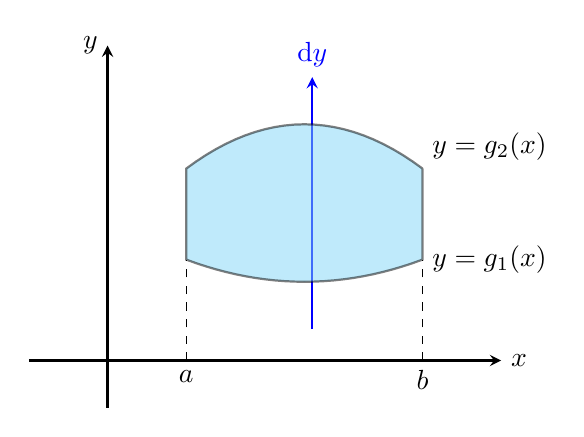
\begin{tikzpicture}[scale=2]
  \draw[thick,->,>=stealth] (-0.5,0.5) -- (2.5,0.5);
  \node[right] at (2.5,0.5) {$x$};
  \draw[thick,->,>=stealth] (0,0.2) -- (0,2.5);
  \node[left] at (0,2.5) {$y$};
  \draw[blue,thick,->,>=stealth] (1.3,0.7) -- (1.3,2.3);
  \node[above,blue] at (1.3,2.3) {$\text{d}y$};
  \draw[black,thick,fill=cyan!50,opacity=0.5]
    plot[domain=0.5:2.0] ({\x},{1+0.25*(\x-1.25)*(\x-1.25)}) -- (2, 1.141) -- (2,1.72) --
    plot[domain=2.0:0.5] ({\x},{2-0.5*(\x-1.25)*(\x-1.25)}) -- cycle;
  \node[below] at (0.5,0.5) {$a$};
  \node[below] at (2.0,0.5) {$b$};
  \draw[dashed] (0.5,0.5) -- (0.5,1.14);
  \draw[dashed] (2,0.5) -- (2,1.14);
  \node[right] at (2,1.14) {$y = g_1(x)$};
  \node[right] at (2,1.86) {$y = g_2(x)$};
\end{tikzpicture}
\end{minipage}
\quad
\begin{minipage}{0.6\textwidth}
  $\ds\int_\Omega f(x, y)\,\text{d}A = \int_a^b\!\int_{g_1(x)}^{g_2(x)}f(x, y)\,\text{d}y\,\text{d}x$
\end{minipage}

\quad

\begin{minipage}{0.4\textwidth}
  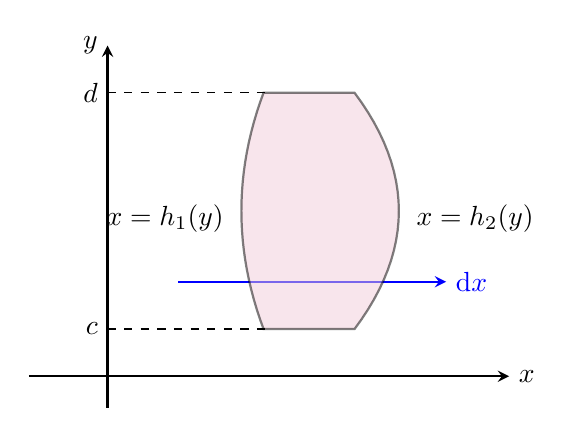
\begin{tikzpicture}[scale=2]
    \draw[thick,->,>=stealth] (-1.05,0.2) --(2,0.2);
    \node[right] at (2,0.2) {$x$};
    \draw[thick,->,>=stealth] (-0.55,-0) -- (-0.55,2.3);
    \node[left]	at (-0.55,2.3) {$y$};
    \draw[blue,thick,->,>=stealth] (-0.1,0.8) -- (1.6,0.8);
    \node[right,blue] at (1.6,0.8) {$\text{d}x$};
    \draw[black,thick,fill=purple!20,opacity=0.5]
    plot[domain=0.5:2.0] ({0.3 + 0.25*(\x-1.25)*(\x-1.25)},{\x}) -- 
    plot[domain=2.0:0.5] ({1.3 - 0.5*(\x-1.25)*(\x-1.25)},{\x}) -- cycle;
    \node[left] at (-0.55,0.5) {$c$};
    \node[left]	at (-0.55,2) {$d$};
    \draw[dashed] (-0.55,0.5) -- (0.5,0.5);
    \draw[dashed] (-0.55,2) -- (0.5,2);
    \node[left] at (0.25,1.2) {$x = h_1(y)$};
    \node[right] at (1.35,1.2) {$x = h_2(y)$};
  \end{tikzpicture}
\end{minipage}
\quad
\begin{minipage}{0.6\textwidth}
  $\ds\int_\Omega f(x, y)\,\text{d}A = \int_c^d\!\int_{h_1(y)}^{h_2(y)}f(x, y)\,\text{d}x\,\text{d}y$
\end{minipage}

\quad

\begin{minipage}{0.25\textwidth}
  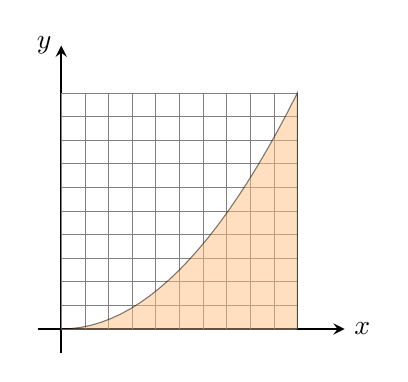
\begin{tikzpicture}[scale=3]
    \draw[thick,->,>=stealth] (-0.1,0) -- (1.2,0);
    \node[right] at (1.2,0) {$x$};
    \draw[thick,->,>=stealth] (0,-0.1) -- (0,1.2);
    \node[left] at (0,1.2) {$y$};
    \draw[help lines,step=0.1] (0,0) grid (1,1);
    \draw[black,fill=orange!50,opacity=0.5] plot[domain=0:1] ({\x},{\x*\x}) -- ++(0,-1)	-- ++(-1,0);
  \end{tikzpicture}
\end{minipage}
\quad
\begin{minipage}{0.75\textwidth}
\begin{ex}
  求 $\ds\int_\Omega x\cos y\,\text{d}A$, $\Omega$ 為 $y = 0$, $x = 1$, 與 $y = x^2$ 圍成之區域.
\end{ex}
\begin{sol}
  $\ds\int_\Omega x\cos y\,\text{d}A = \int_0^1\!\int_0^{x^2}\!\!x\cos y\,\text{d}y\,\text{d}x = \int_0^1\!\!x\,\Big(\sin y\,\Big|_0^{x^2}\Big)\,\text{d}x \\ = \int_0^1 x\sin x^2\,\text{d}x = \frac{1 - \cos 1}{2}$
\end{sol}
\end{minipage}

\quad

\begin{minipage}{0.25\textwidth}
  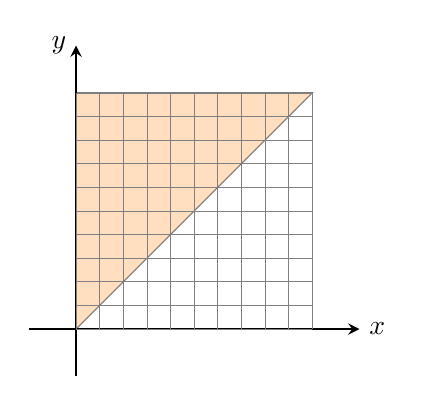
\begin{tikzpicture}[scale=3]
    \draw[thick,->,>=stealth] (-0.2,0) -- (1.2,0);
    \node[right] at (1.2,0) {$x$};
    \draw[thick,->,>=stealth] (0,-0.2) -- (0,1.2);
    \node[left] at (0,1.2) {$y$};
    \draw[black,fill=orange!50,opacity=0.5]  (0,0) -- (1,1) -- (0,1) -- cycle; 
    \draw[help lines,step=0.1] (0,0) grid (1,1);
  \end{tikzpicture}
\end{minipage}
\quad
\begin{minipage}{0.75\textwidth}
\begin{ex}
  求 $\ds\int_\Omega e^{-y^2}\,\text{d}A$, $\Omega = \{(x,\,y)\,|\,0\leqslant y\leqslant 1,\;0\leqslant x\leqslant y\}$.
\end{ex}
\begin{sol}
  $\ds\int_\Omega e^{-y^2}\,\text{d}A = \int_0^1\!\int_0^y e^{-y^2}\,\text{d}x\,\text{d}y = \int_0^1\!ye^{-y^2}\,\text{d}y = \frac{1 - e^{-1}}{2}$
\end{sol}
\end{minipage}

\quad

\begin{minipage}{0.25\textwidth}
  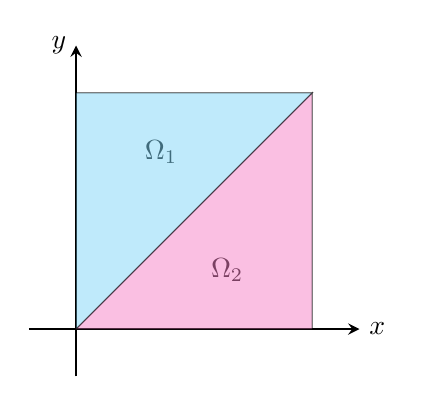
\begin{tikzpicture}[scale=3]
    \draw[thick,->,>=stealth] (-0.2,0) -- (1.2,0);
    \node[right] at (1.2,0) {$x$};
    \draw[thick,->,>=stealth] (0,-0.2) -- (0,1.2);
    \node[left] at (0,1.2) {$y$};
    \node[right] at (0.25,0.75) {$\Omega_1$};
    \node[left] at (0.75,0.25) {$\Omega_2$};
    \draw[black,fill=cyan!50,opacity=0.5]  (0,0) -- (1,1) -- (0,1) -- cycle; 
    \draw[black,fill=magenta!50,opacity=0.5]  (0,0) -- (1,1) -- (1,0) -- cycle; 
    %\draw[help lines,step=0.1] (0,0) grid (1,1);
  \end{tikzpicture}
\end{minipage}
\quad
\begin{minipage}{0.75\textwidth}
\begin{ex}
  求 $\ds\int_0^1\!\int_0^1\!e^{\max\{x^2,\,y^2\}}\,\text{d}x\,\text{d}y$.
\end{ex}
\begin{sol}
  $\ds\int_0^1\!\int_0^1\!e^{\max\{x^2,\,y^2\}}\,\text{d}x\,\text{d}y = \int_{\Omega_1} e^{y^2}\,\text{d}A + \int_{\Omega_2} e^{x^2}\,\text{d}A \\ = \int_0^1\!\int_0^y e^{y^2}\,\text{d}x\,\text{d}y + \int_0^1\!\int_0^x e^{x^2}\,\text{d}y\,\text{d}x = \int_0^1\!ye^{y^2}\,\text{d}y + \int_0^1\!xe^{x^2}\,\text{d}x = e - 1$.
\end{sol}
\end{minipage}

\subsection*{積分順序交換}
\quad
\begin{minipage}{0.25\textwidth}
  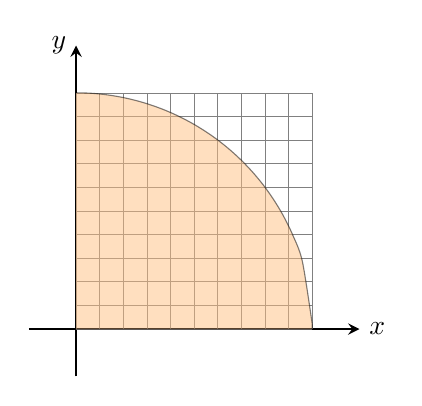
\begin{tikzpicture}[scale=3]
    \draw[thick,->,>=stealth] (-0.2,0) -- (1.2,0);
    \node[right] at (1.2,0) {$x$};
    \draw[thick,->,>=stealth] (0,-0.2) -- (0,1.2);
    \node[left] at (0,1.2) {$y$};
    \draw[help lines,step=0.1] (0,0) grid (1,1);
    \draw[black,fill=orange!50,opacity=0.5] plot[domain=0:1,smooth] ({\x},{sqrt(1 - \x*\x)}) -- (1,0) -- (0,0);
  \end{tikzpicture}
\end{minipage}
\quad
\begin{minipage}{0.75\textwidth}
\begin{ex}
  求 $\ds\int_0^1\!\int_0^{\sqrt{1 - x^2}}\!\!\!\!\!\!\sqrt{1 - y^2}\,\text{d}y\,\text{d}x$.
\end{ex}
\begin{sol}
  $\ds\int_0^1\!\int_0^{\sqrt{1 - x^2}}\!\!\!\!\!\!\sqrt{1 - y^2}\,\text{d}y\,\text{d}x = \int_0^1\!\int_0^{\sqrt{1 - y^2}}\!\!\!\!\!\!\sqrt{1 - y^2}\,\text{d}x\,\text{d}y = \int_0^1\!(1 - y^2)\,\text{d}y = \frac{2}{3}$. \\ $\ds\int_0^1\!\int_0^{\sqrt{1 - x^2}}\!\!\!\!\!\!\sqrt{1 - y^2}\,\text{d}y\,\text{d}x = \frac{1}{2}\int_0^1(\sin^{-1}\!\sqrt{1 - x^2} + x\sqrt{1 - x^2})\,\text{d}x = \frac{1}{2}\,\Big(1 + \frac{1}{3}\Big) = \frac{2}{3}$.
\end{sol}
\end{minipage}

\begin{ex} 將下列積分以不同積分順序寫出. 
  \begin{multicols}{2}
    \begin{enumerate}\setlength{\itemsep}{0pt}
      \item $\ds\int_0^2\!\int_{x^2}^{2x}\!f(x, y)\,\text{d}y\,\text{d}x$
      \item $\ds\int_0^1\!\int_{\sin^{-1}y}^{\frac{\pi}{2}}\!f(x, y)\,\text{d}x\,\text{d}y$
      \item $\ds\int_{-1}^2\!\int_{x^2}^{x + 2}\!f(x, y)\,\text{d}y\,\text{d}x$
      \item $\ds\int_0^1\!\int_0^{2y}\!f(x, y)\,\text{d}x\,\text{d}y$ + $\ds\int_1^3\!\int_0^{3 - y}\!f(x, y)\,\text{d}x\,\text{d}y$
    \end{enumerate}
  \end{multicols}
\end{ex}

\begin{sol}
  \begin{enumerate}\setlength{\itemsep}{0pt}
    \item[]
    \item $\ds\int_0^2\!\int_{x^2}^{2x}\!f(x, y)\,\text{d}y\,\text{d}x = \int_0^4\!\int_{\sqrt{y}}^{\frac{y}{2}}\!f(x, y)\,\text{d}x\,\text{d}y$
    \item $\ds\int_0^1\!\int_{\sin^{-1}y}^{\frac{\pi}{2}}\!f(x, y)\,\text{d}x\,\text{d}y = \int_0^{\frac{\pi}{2}}\!\int_0^{\sin x}\!f(x, y)\,\text{d}x\,\text{d}y$
    \item $\ds\int_{-1}^2\!\int_{x^2}^{x + 2}\!f(x, y)\,\text{d}y\,\text{d}x = \int_0^1\!\int_{-\sqrt{y}}^{\sqrt{y}}\!f(x, y)\,\text{d}x\,\text{d}y + \int_1^4\!\int_{y - 2}^{\sqrt{y}}\!f(x, y)\,\text{d}x\,\text{d}y$
    \item $\ds\int_0^1\!\int_0^{2y}\!f(x, y)\,\text{d}x\,\text{d}y + \int_1^3\!\int_0^{3 - y}\!f(x, y)\,\text{d}x\,\text{d}y = \int_0^2\!\int_{\frac{x}{2}}^{3 - x}\!f(x, y)\,\text{d}y\,\text{d}x$
  \end{enumerate}
\end{sol}

\begin{ex}
  證明 $\ds\int_0^x\!\int_0^t F(u)\,\text{d}u\,\text{d}t = \int_0^x(x - u)F(u)\,\text{d}u$.
\end{ex}

\begin{sol}
  $\ds\int_0^x\!\int_0^t F(u)\,\text{d}u\,\text{d}t = \int_0^x\!\int_u^x F(u)\,\text{d}t\,\text{d}u = \int_0^x(x - u)F(u)\,\text{d}u$.
\end{sol}

\begin{ex}
  求 $\ds\int_0^1\!\int_x^1 e^{-y^2}\,\text{d}y\,\text{d}x$.
\end{ex}

\begin{sol}
  $\ds\int_0^1\!\int_x^1 e^{-y^2}\,\text{d}y\,\text{d}x = \int_0^1\!\int_0^y e^{-y^2}\,\text{d}x\,\text{d}y = \int_0^1\!ye^{-y^2}\,\text{d}y = \frac{1 - e^{-1}}{2}$
\end{sol}

\begin{ex}
  求 $\ds\int_0^1\!\int_y^1\frac{\sin x}{x}\,\text{d}x\,\text{d}y$.
\end{ex}

\begin{sol}
  $\ds\int_0^1\!\int_y^1\frac{\sin x}{x}\,\text{d}x\,\text{d}y = \int_0^1\!\int_0^x\frac{\sin x}{x}\,\text{d}y\,\text{d}x = \int_0^1\!\sin x\,\text{d}x = 1 - \cos 1$.
\end{sol}

\begin{ex}
  求 $\ds\int_0^1\!\int_{\sin^{-1}\!y}^{\frac{\pi}{2}}\!\!\!\cos x\,\sqrt{1 + \cos^2 x}\,\text{d}x\,\text{d}y$.
\end{ex}

\begin{sol}
  \begin{itemize}\setlength{\itemsep}{0pt}
    \item[]
    \item $\ds\int_0^1\!\int_{\sin^{-1}\!y}^{\frac{\pi}{2}}\!\!\!\cos x\,\sqrt{1 + \cos^2 x}\,\text{d}x\,\text{d}y = \int_0^{\frac{\pi}{2}}\!\int_0^{\sin x}\!\!\!\cos x\,\sqrt{1 + \cos^2 x}\,\text{d}y\,\text{d}x = \int_0^{\frac{\pi}{2}}\!\sin x\cos x\sqrt{1 + \cos^2 x}\,\text{d}x \\= \int_0^1\!u\sqrt{1 + u^2}\,\text{d}u = \int_1^2\!\!\sqrt{v}\,\frac{1}{2}\,\text{d}v = \frac{2\sqrt{2} - 1}{3}$, 其中變數變換 $u = \cos x$ 與 $v = 1 + u^2$. 
    \item 令 $u = \sin x$, $\ds\int_{\sin^{-1}y}^{\frac{\pi}{2}}\!\!\!\cos x\,\sqrt{1 + \cos^2 x}\,\text{d}x = \int_y^1\!\sqrt{2 - u^2}\,\text{d}u$. 令 $u = \sqrt{2}\sin\theta$, 則 $\ds\int_y^1\!\sqrt{2 - u^2}\,\text{d}u = \int_{\sin^{-1}\!\!\frac{y}{\sqrt{2}}}^{\frac{\pi}{4}}2\cos^2\theta\,\text{d}\theta = \int_{\sin^{-1}\!\!\frac{y}{\sqrt{2}}}^{\frac{\pi}{4}}(1 + \cos2\theta)\,\text{d}\theta = (\theta + \sin\theta\cos\theta)\,\Big|_{\sin^{-1}\!\!\frac{y}{\sqrt{2}}}^{\frac{\pi}{4}} = \frac{\pi}{4} + \frac{1}{2} - \sin^{-1}\!\!\frac{y}{\sqrt{2}} - \frac{y}{\sqrt{2}}\cdot\frac{\sqrt{2 - y^2}}{\sqrt{2}} = \frac{\pi}{4} + \frac{1}{2} - \sin^{-1}\!\!\frac{y}{\sqrt{2}} - \frac{y\sqrt{2 - y^2}}{2}$. 故 $\ds\int_0^1\!\int_{\sin^{-1}y}^{\frac{\pi}{2}}\!\!\!\cos x\,\sqrt{1 + \cos^2 x}\,\text{d}x\,\text{d}y \\= \int_0^1\!\bigg(\frac{\pi}{4} + \frac{1}{2} - \sin^{-1}\!\!\frac{y}{\sqrt{2}} - \frac{y\sqrt{2 - y^2}}{2}\bigg)\,\text{d}y = \frac{\pi}{4} + \frac{1}{2} - \Big(\frac{\pi}{4} + 1 - \sqrt{2}\Big) - \Big(\frac{\sqrt{2}}{3} - \frac{1}{6}\Big) = \frac{2\sqrt{2} - 1}{3}$. 
  \end{itemize}
\end{sol}

\begin{ex}
  求 $\ds\int_0^\infty\frac{e^{-ax} - e^{-bx}}{x}\,\text{d}x$, $b > a > 0$. 
\end{ex}

\begin{sol}
  由 $\ds\int_a^b\!e^{-xy}\,\text{d}y = \frac{1}{-x}e^{-xy}\,\Big|_{y=a}^{y=b} = \frac{1}{-x}(e^{-xb} - e^{-xa}) = \frac{e^{-ax} - e^{-bx}}{x}$, $\ds\int_0^\infty\!\frac{e^{-ax} - e^{-bx}}{x}\,\text{d}x = \int_0^\infty\!\bigg(\int_a^b\!e^{-xy}\,\text{d}y\bigg)\,\text{d}x = \int_a^b\!\bigg(\int_0^\infty e^{-xy}\,\text{d}x\bigg)\,\text{d}y = \int_a^b\frac{1}{y}\,\text{d}y = \ln\frac{b}{a}$. 
\end{sol}

\begin{ex}
  求 $\ds\int_0^\infty\!\frac{\tan^{-1}\pi x - \tan^{-1}x}{x}\,\text{d}x$. 
\end{ex}

\begin{sol}
  由 $\ds\int_{x}^{\pi x}\!\!\frac{1}{1 + y^2}\,\text{d}y = \tan^{-1}\pi x - \tan^{-1}x$, $\ds\int_0^\infty\frac{\tan^{-1}\pi x - \tan^{-1}x}{x}\,\text{d}x = \int_0^\infty\!\frac{1}{x}\bigg(\int_{x}^{\pi x}\!\!\frac{1}{1 + y^2}\,\text{d}y\bigg)\,\text{d}x \\= \int_0^\infty\!\!\int_{x}^{\pi x}\!\!\frac{1}{x\,(1 + y^2)}\,\text{d}y\,\text{d}x = \int_0^\infty\!\!\int_{\frac{y}{\pi}}^{y}\!\!\frac{1}{x\,(1 + y^2)}\,\text{d}x\,\text{d}y = \int_0^\infty\!\!\frac{1}{1 + y^2}\bigg(\int_{\frac{y}{\pi}}^{y}\frac{1}{x}\,\text{d}x\bigg)\,\text{d}y = \int_0^\infty\!\!\frac{1}{1 + y^2}\Big(\ln y - \ln\frac{y}{\pi}\Big)\,\text{d}y = \int_0^\infty\!\!\frac{\ln\pi}{1 + y^2}\,\text{d}y = \frac{\pi}{2}\ln\pi$.
\end{sol}

\begin{ex}
  求 $\ds\int_0^\infty\frac{\sin x}{x}\,\text{d}x$. 
\end{ex}

\begin{sol}
  由 $\ds\int_0^\infty\!e^{-xy}\,\text{d}y = \frac{1}{x}$, $x > 0$; 又 $\ds\int\!e^{ax}\sin bx\,\text{d}x = \frac{e^{ax}(a\cdot\sin bx - b\cdot\cos bx)}{a^2 + b^2}$. \\故 $\ds\int_0^\infty\!\frac{\sin x}{x}\,\text{d}x = \int_0^\infty\!\sin x\,\bigg(\int_0^\infty\!e^{-xy}\,\text{d}y\bigg)\,\text{d}x = \int_0^\infty\!\!\bigg(\int_0^\infty\!e^{-xy}\sin x\,\text{d}y\bigg)\,\text{d}x = \int_0^\infty\!\!\bigg(\int_0^\infty\!e^{-xy}\sin x\,\text{d}x\bigg)\,\text{d}y = \int_0^\infty\!\frac{e^{-xy}((-y)\cdot\sin x - 1\cdot\cos x)}{(-y)^2 + 1^2}\,\Big|_{x = 0}^{x = \infty}\,\text{d}y = \int_0^\infty\!\frac{0 - (-1)}{1 + y^2}\,\text{d}y = \int_0^\infty\!\frac{1}{1 + y^2}\,\text{d}y = \tan^{-1}y\,\Big|_{0}^{\infty} = \frac{\pi}{2}$. 
\end{sol}

%\begin{ex}[Fubini 定理之反例]
%  求 $\ds\int_0^1\!\int_0^1\!\frac{x - y}{(x + y)^3}\,\text{d}y\,\text{d}x$ 與 $\ds\int_0^1\!\int_0^1\!\frac{x - y}{(x + y)^3}\,\text{d}x\,\text{d}y$.
%\end{ex}
%
%\begin{sol}
%  \begin{itemize}\setlength{\itemsep}{0pt}
%    \item[]
%    \item 令 $\ds t = x + y$, 則 $\ds y = t - x,\;\text{d}y = \text{d}t$, $y$ 由 $0$ 到 $1$, $t = x + y$ 由 $x + 0 = x$ 到 $x + 1$, $\ds\int_0^1\!\frac{x - y}{(x + y)^3}\,\text{d}y = \int_{x}^{x + 1}\frac{2x - t}{t^3}\,\text{d}t = \Big(-\frac{x}{t^2} + \frac{1}{t}\Big)\,\Big|_x^{x + 1} = \frac{1}{(x + 1)^2}$; 故 $\ds\int_0^1\!\int_0^1\!\frac{x - y}{(x + y)^3}\,\text{d}y\,\text{d}x = \int_0^1\!\frac{1}{(x + 1)^2}\,\text{d}x = \frac{1}{2}$. 
%    \item 令 $\ds t = x + y$, 則 $\ds x = t - y,\;\text{d}x = \text{d}t$, $x$ 由 $0$ 到 $1$, $t = x + y$ 由 $y + 0 = y$ 到 $y + 1$, $\ds\int_0^1\!\frac{x - y}{(x + y)^3}\,\text{d}x = \int_{y}^{y + 1}\frac{t - 2y}{t^3}\,\text{d}t = \Big(-\frac{1}{t} + \frac{y}{t^2}\Big)\,\Big|_y^{y + 1} = -\frac{1}{(y + 1)^2}$; 故 $\ds\int_0^1\!\int_0^1\!\frac{x - y}{(x + y)^3}\,\text{d}x\,\text{d}y = -\int_0^1\!\frac{1}{(y + 1)^2}\,\text{d}x = -\frac{1}{2}$. 
%  \end{itemize}
%\end{sol}

\subsection*{變數變換}
單變數積分 $\ds\int_{[a,\,b]}\!f(x)\,\text{d}x$ 中, 令 $\ds x = x(u)$, 則 $\ds\text{d}x = \frac{\text{d}x}{\text{d}u}\,\text{d}u$; $\ds\int_{[a,\,b]}\!f(x)\,\text{d}x = \underbrace{\int_{x^{-1}[a, b]}}_{\text{由小到大}}\!f(x(u))\,\bigg|\frac{\text{d}x}{\text{d}u}\bigg|\,\text{d}u$. 
\begin{ex}
  \begin{itemize}\setlength{\itemsep}{0pt}
    \item[]
    \item 求 $\ds\int_0^{1}\!\frac{\text{d}x}{\sqrt{1 - x^2}}$: 令 $\ds x = \sin u$, 則 $\ds\text{d}x = \cos u\cdot\text{d}u$; $x$ 由 $\ds 0$ 至 $\ds 1$, 則 $u$ 由 $\ds\sin^{-1}0 = 0$ 至 $\ds\sin^{-1}1 = \frac{\pi}{2}$. 故 $\ds\int_0^{1}\!\frac{\text{d}x}{\sqrt{1 - x^2}} = \int_0^{\frac{\pi}{2}}\!\frac{\cos u\cdot\text{d}u}{\sqrt{1 - \sin^2 u}} = \int_0^{\frac{\pi}{2}}\!\frac{\cos u\cdot\text{d}u}{\cos u} = \int_0^{\frac{\pi}{2}}\!1\cdot\text{d}u = \frac{\pi}{2}$.
    \item 求 $\ds\int_{\frac{1}{2}}^1\!(1 - 2x)^2\,\text{d}x$: 令 $\ds u = 1 - 2x$, 亦即 $\ds x = \frac{1}{2} - \frac{u}{2}$, 則 $\ds\text{d}x = \frac{-1}{2}\,\text{d}u$; $x$ 由 $\ds\frac{1}{2}$ 至 $1$, 則 $u$ 由 $\ds 1 - 2\cdot\frac{1}{2} = 0$ 至 $1 - 2\cdot 1 = -1$. 故 $\ds\int_{\frac{1}{2}}^1\!(1 - 2x)^2\,\text{d}x = \int_0^{-1}\!u^2\,\Big(\frac{-1}{2}\Big)\,\text{d}u = \int_{-1}^0\!u^2\,\frac{1}{2}\,\text{d}u = \frac{1}{6}$. 
  \end{itemize}
\end{ex}

\begin{thm}[重積分變數變換]
  給定 $\Omega_{\vx},\,\Omega_{\vu}\subseteq\mathbb{R}^n$, $\ds\vx = \vx(\vu):\,\Omega_{\vu}\to\Omega_{\vx}$ 且 
  \begin{itemize}
    \item $\vx$ 為嵌射 (亦即 $\ds\vx(\Omega_{\vu}) = \Omega_{\vx},\;\vx^{-1}(\Omega_{\vx}) = \Omega_{\vu}$)
    \item $\vx$ 之各分量函數 $x_j$, $j = 1,\,2\,\ldots,\,n$ 為連續可偏微分
    \item $\forall\,\vu\in\Omega_{\vu}$, $\vx$ 之 Jacobian $\ds J_{\vx}(\vu) = \frac{\partial\vx}{\partial\vu}(\vu) = \begin{vmatrix}\frac{\partial x_1}{\partial u_1} & \frac{\partial x_1}{\partial u_n} & \ldots &\frac{\partial x_1}{\partial u_n} \\ \frac{\partial x_2}{\partial u_1}& \frac{\partial x_2}{\partial u_n} & \ldots &\frac{\partial x_2}{\partial u_n} \\ \vdots & \vdots & \ddots & \vdots \\ \frac{\partial x_n}{\partial u_1} & \frac{\partial x_n}{\partial u_n} & \ldots &\frac{\partial x_n}{\partial u_n} \end{vmatrix}(\vu)\ne 0$
  \end{itemize}
  則對於可積函數 $f:\Omega_{\vx}\to\mathbb{R}$, $\ds\int_{\Omega_{\vx}} f(\vx)\,\text{d}\vx = \int_{\vx^{-1}(\Omega_{\vx})}\!\!\!\!f(\vx(\vu))\,\big|J_{\vx}(\vu)\big|\,\text{d}\vu = \int_{\vx^{-1}(\Omega_{\vx})}\!\!\!\!f(\vx(\vu))\,\bigg|\frac{\partial\vx}{\partial\vu}\bigg|\,\text{d}\vu$.
\end{thm}

\begin{ex}
  利用變數變換 $x = u^2 - v^2$, $y = 2uv$ 求 $\ds\int_\Omega\!y\,\text{d}A$, $\Omega$ 為 $y \geqslant 0$, $y^2 = 4 - 4x$, $y^2 = 4  + 4x$ 所圍成之區域. 
\end{ex}

\begin{sol}
  由 $\ds\begin{cases}x = u^2 - v^2 \\ y = 2uv\end{cases}\!\!\!\!\!$, Jacobian $\ds J_{\vx}(\vu) = \frac{\partial\vx}{\partial\vu}(\vu) = \begin{vmatrix}\frac{\partial x}{\partial u} & \frac{\partial x}{\partial v} \\ \frac{\partial y}{\partial u}& \frac{\partial y}{\partial v}\end{vmatrix} = \begin{vmatrix}2u & -2v\\ 2v & 2u\end{vmatrix} = 4\,(u^2 + v^2)$. 變數變換 $(x,\,y)\to(u,\,v)$ 後 $\Omega$ 由 $uv = 0$, $u^2v^2 + u^2 - v^2 - 1 = (v^2 + 1)(u^2 - 1) = 0$, $u^2v^2 - u^2 + v^2 - 1 = (u^2 + 1)(v^2 - 1) = 0$ 圍成, 亦即 $\Omega = \{0\leqslant u\leqslant 1,\;0\leqslant v\leqslant 1\}$, 故 $\ds\int_\Omega\!y\,\text{d}A = \int_0^1\!\int_0^1 2uv\,\Big|4\,(u^2 + v^2)\Big|\,\text{d}u\,\text{d}v = 2$.
\end{sol}

\begin{ex}
  求 $\ds\int_\Omega\!(x + y)^2\,\text{d}A$, $\Omega$ 為 $x + y = 0$, $x + y = 1$, $2x - y = 0$, $2x - y = 3$ 所圍成之平行四邊形. 
\end{ex}

\begin{sol}
  令 $\ds\begin{cases}u = x + y \\ v = 2x - y\end{cases}\!\!\!\!\!$, 則 $\ds\begin{cases}x = \frac{1}{3}u + \frac{1}{3}v \\ y = \frac{2}{3}u - \frac{1}{3}v\end{cases}\!\!\!\!\!$; Jacobian $\ds J_{\vx}(\vu) = \frac{\partial\vx}{\partial\vu}(\vu) = \begin{vmatrix}\frac{\partial x}{\partial u} & \frac{\partial x}{\partial v} \\ \frac{\partial y}{\partial u}& \frac{\partial y}{\partial v}\end{vmatrix} = \begin{vmatrix}\frac{1}{3} & \frac{1}{3} \\ \frac{2}{3} & \frac{-1}{3}\end{vmatrix} = -\frac{1}{3}$. 變數變換 $(x,\,y)\to(u,\,v)$ 後 $\Omega = \{0\leqslant u\leqslant 1,\;0\leqslant v\leqslant 3\}$, 故 $\ds\int_\Omega\!(x + y)^2\,\text{d}A = \int_0^3\!\int_0^1 u^2\,\Big|-\frac{1}{3}\Big|\,\text{d}u\,\text{d}v = \frac{1}{3}$.
\end{sol}

\begin{ex}
  求 $\ds\int_\Omega\!\sqrt{x + y}\;\text{d}A$, $\Omega$ 為頂點 $(0,\,0),\;(a,\,0),\;(0,\,a)$, $a > 0$ 之三角形. 
\end{ex}

\begin{sol}
  令 $\ds\begin{cases}u = x + y \\ v = x - y\end{cases}\!\!\!\!\!$, 則 $\ds\begin{cases}x = \frac{1}{2}u + \frac{1}{2}v \\ y = \frac{1}{2}u - \frac{1}{2}v\end{cases}\!\!\!\!\!$; Jacobian $\ds J_{\vx}(\vu) = \frac{\partial\vx}{\partial\vu}(\vu) = \begin{vmatrix}\frac{\partial x}{\partial u} & \frac{\partial x}{\partial v} \\ \frac{\partial y}{\partial u}& \frac{\partial y}{\partial v}\end{vmatrix} = \begin{vmatrix}\frac{1}{2} & \frac{1}{2} \\ \frac{1}{2} & \frac{-1}{2}\end{vmatrix} = -\frac{1}{2}$. 變數變換前 $\Omega$ 由 $x + y = 0$, $x + y = a$, $x = 0$, $y = 0$ 所圍成, 變數變換 $(x,\,y)\to(u,\,v)$ 後 $\Omega$ 由 $u = 0$, $u = a$, $u + v = 0$, $u - v = 0$ 圍成, 故 $\ds\int_\Omega\!\sqrt{x + y}\;\text{d}A = \int_0^a\!\int_{-u}^{u}\!\sqrt{u}\,\Big|-\frac{1}{2}\Big|\,\text{d}v\,\text{d}u = \int_0^a\!u\sqrt{u}\,\text{d}u = \frac{2\,a^{\frac{5}{2}}}{5}$.
\end{sol}

\begin{ex}
  求 $\ds\int_\Omega\!(x + y)\,e^{x - y}\,\text{d}A$, $\Omega$ 為頂點 $(4,\,0),\;(6,\,2),\;(4,\,4),\;(2,\,2)$ 之四邊形. 
\end{ex}

\begin{sol}
  令 $\ds\begin{cases}u = x + y \\ v = x - y\end{cases}\!\!\!\!\!$, 則 $\ds\begin{cases}x = \frac{1}{2}u + \frac{1}{2}v \\ y = \frac{1}{2}u - \frac{1}{2}v\end{cases}\!\!\!\!\!$; Jacobian $\ds J_{\vx}(\vu) = \frac{\partial\vx}{\partial\vu}(\vu) = \begin{vmatrix}\frac{\partial x}{\partial u} & \frac{\partial x}{\partial v} \\ \frac{\partial y}{\partial u}& \frac{\partial y}{\partial v}\end{vmatrix} = \begin{vmatrix}\frac{1}{2} & \frac{1}{2} \\ \frac{1}{2} & \frac{-1}{2}\end{vmatrix} = -\frac{1}{2}$. 變數變換前 $\Omega$ 由 $x - y = 0$, $x - y = 4$, $x + y = 4$, $x + y = 8$ 所圍成, 變數變換 $(x,\,y)\to(u,\,v)$ 後 $\Omega$ 由 $v = 0$, $v = 4$, $u = 4$, $u = 8$ 圍成, 故 $\ds\int_\Omega\!(x + y)\,e^{x - y}\,\text{d}A = \int_0^4\!\int_4^8 ue^v\Big|-\frac{1}{2}\Big|\,\text{d}u\,\text{d}v = \frac{1}{2}\int_0^4 e^v\,\text{d}v\!\int_4^8 u\,\text{d}u = 12\,(e^4 - 1)$.
\end{sol}

\begin{ex}
  求 $\ds\int_\Omega\!e^{\frac{x + y}{x - y}}\,\text{d}A$, $\Omega$ 為頂點 $(1,\,0),\;(2,\,0),\;(0,\,-2),\;(0,\,-1)$ 之梯形. 
\end{ex}

\begin{sol}
  令 $\ds\begin{cases}u = x + y \\ v = x - y\end{cases}\!\!\!\!\!$, 則 $\ds\begin{cases}x = \frac{1}{2}u + \frac{1}{2}v \\ y = \frac{1}{2}u - \frac{1}{2}v\end{cases}\!\!\!\!\!$; Jacobian $\ds J_{\vx}(\vu) = \frac{\partial\vx}{\partial\vu}(\vu) = \begin{vmatrix}\frac{\partial x}{\partial u} & \frac{\partial x}{\partial v} \\ \frac{\partial y}{\partial u}& \frac{\partial y}{\partial v}\end{vmatrix} = \begin{vmatrix}\frac{1}{2} & \frac{1}{2} \\ \frac{1}{2} & \frac{-1}{2}\end{vmatrix} = -\frac{1}{2}$. 變數變換前 $\Omega$ 由 $x - y = 1$, $x - y = 2$, $x = 0$, $y = 0$ 所圍成, 變數變換 $(x,\,y)\to(u,\,v)$ 後 $\Omega$ 由 $v = 1$, $v = 2$, $u + v = 0$, $u - v = 0$ 圍成, 故 $\ds\int_\Omega\!e^{\frac{x + y}{x - y}}\,\text{d}A = \int_1^2\!\int_{-v}^{v} e^{\frac{u}{v}}\,\Big|-\frac{1}{2}\Big|\,\text{d}u\,\text{d}v = \frac{1}{2}\,\int_1^2\!\Big(v\,e^{\frac{u}{v}}\,\Big|_{u = -v}^{u = v}\Big)\,\text{d}v = \frac{3\,(e - e^{-1})}{4}$.
\end{sol}

\begin{ex}
  求 $y = x^2$, $y = 2x^2$, $x = y^2$, $x = 3y^2$ 所圍成之區域面積. 
\end{ex}

\begin{sol}
  令 $\ds\begin{cases}u = \frac{y}{x^2} \\ v = \frac{x}{y^2}\end{cases}\!\!\!\!\!$, 則 $\ds\begin{cases}x = (u^2 v)^{-\frac{1}{3}} \\ y = (u v^2)^{-\frac{1}{3}} \end{cases}\!\!\!\!\!$; Jacobian $\ds J_{\vx}(\vu) = \frac{\partial\vx}{\partial\vu}(\vu) = \begin{vmatrix}\frac{\partial x}{\partial u} & \frac{\partial x}{\partial v} \\ \frac{\partial y}{\partial u}& \frac{\partial y}{\partial v}\end{vmatrix} = \begin{vmatrix}-\frac{1}{3}(u^2 v)^{-\frac{4}{3}}\cdot 2uv & -\frac{1}{3}(u^2 v)^{-\frac{4}{3}}\cdot u^2\\ -\frac{1}{3}(u v^2)^{-\frac{4}{3}}\cdot v^2 & -\frac{1}{3}(u v^2)^{-\frac{4}{3}}\cdot 2uv\end{vmatrix}\\ = \frac{1}{3u^2v^2}$. 變數變換 $(x,\,y)\to(u,\,v)$ 後 $\Omega$ 由 $u = 1$, $u = 2$, $v = 1$, $v = 3$ 圍成, 亦即 $\Omega = \{1\leqslant u\leqslant 2,\;1\leqslant v\leqslant 3\}$, 面積為 $\ds\int_\Omega\!\text{d}A = \int_1^3\!\int_1^2\bigg|\frac{1}{3u^2v^2}\bigg|\,\text{d}u\,\text{d}v = \frac{1}{9}$.
\end{sol}

\begin{ex}
  求 $\ds\int_\Omega\frac{xy}{1 + x^2y^2}\,\text{d}A$, $\Omega$ 為 $xy = 1$, $xy = 5$, $x = 1$, $x = 6$ 所圍成之區域. 
\end{ex}

\begin{sol}
  令 $\ds\begin{cases}u = xy \\ v = x\end{cases}\!\!\!\!\!$, 則 $\ds\begin{cases}x = v \\ y = \frac{u}{v} \end{cases}\!\!\!\!\!$; Jacobian $\ds J_{\vx}(\vu) = \frac{\partial\vx}{\partial\vu}(\vu) = \begin{vmatrix}\frac{\partial x}{\partial u} & \frac{\partial x}{\partial v} \\ \frac{\partial y}{\partial u}& \frac{\partial y}{\partial v}\end{vmatrix} = \begin{vmatrix} 0 & 1\\ \frac{1}{v} & -\frac{u}{v^2}\end{vmatrix} = -\frac{1}{v}$. 變數變換 $(x,\,y)\to(u,\,v)$ 後 $\Omega$ 由 $u = 1$, $u = 5$, $v = 1$, $v = 6$ 圍成, 亦即 $\Omega = \{1\leqslant u\leqslant 5,\;1\leqslant v\leqslant 6\}$, 故 $\ds\int_\Omega\!\frac{xy}{1 + x^2y^2}\,\text{d}A = \int_1^6\!\int_1^5\frac{u}{1 + u^2}\,\bigg|-\frac{1}{v}\bigg|\,\text{d}u\,\text{d}v = \int_1^6\!\frac{1}{v}\,\text{d}v\,\int_1^5\frac{u}{1 + u^2}\,\text{d}u = \frac{\ln 6\cdot\ln 13}{2}$.
\end{sol}

\begin{ex}
  求 $\ds\int_\Omega\frac{y}{x}\;\text{d}A$, $\Omega$ 為 $y = x$, $x^2 + 4y^2 = 4$, $y \geqslant 0$ 所圍成之區域. 
\end{ex}

\begin{sol}
  令 $\ds\begin{cases}x = 2r\cos\theta \\ y = r\sin\theta \end{cases}\!\!\!\!\!$, Jacobian $\ds J_{\vx}(\vu) = \frac{\partial\vx}{\partial\vu}(\vu) = \begin{vmatrix}\frac{\partial x}{\partial r} & \frac{\partial x}{\partial\theta} \\ \frac{\partial y}{\partial r}& \frac{\partial y}{\partial\theta}\end{vmatrix} = \begin{vmatrix} 2\cos\theta & -2r\sin\theta\\ \sin\theta & r\cos\theta\end{vmatrix} = 2r$. 變數變換 $(x,\,y)\to(r,\,\theta)$ 後 $\Omega$ 由 $r = 0$, $r = 1$, $\theta = 0$, $\ds\theta = \tan^{-1}2$ 圍成, 亦即 $\Omega = \{0\leqslant r\leqslant 1,\;0\leqslant\theta\leqslant\tan^{-1}2\}$, 故 $\ds\int_\Omega\!\frac{y}{x}\;\text{d}A = \int_0^{\tan^{-1}2}\!\!\!\int_0^1\!\frac{1}{2}\,\tan\theta\,\big|2r\big|\,\text{d}r\,\text{d}\theta = \int_0^{\tan^{-1}2}\!\!\!\!\!\!\tan\theta\,\text{d}\theta\,\int_0^1 r\,\text{d}r = -\frac{1}{2}\,\ln|\cos\theta|\,\bigg|_0^{\tan^{-1}2} = \frac{\ln 5}{4}$.
\end{sol}

\begin{ex}
  求 $\ds\int_\Omega\sin(9x^2 + 4y^2)\;\text{d}A$, $\Omega$ 為 $9x^2 + 4y^2 = 1$, $y\geqslant 0$, $x\geqslant 0$ 所圍成之區域. 
\end{ex}

\begin{sol}
  令 $\ds\begin{cases}x = \frac{1}{3}\,r\cos\theta \\ y = \frac{1}{2}\,r\sin\theta \end{cases}\!\!\!\!\!$, Jacobian $\ds J_{\vx}(\vu) = \frac{\partial\vx}{\partial\vu}(\vu) = \begin{vmatrix}\frac{\partial x}{\partial r} & \frac{\partial x}{\partial\theta} \\ \frac{\partial y}{\partial r}& \frac{\partial y}{\partial\theta}\end{vmatrix} = \begin{vmatrix} \frac{1}{3}\,\cos\theta & -\frac{1}{3}\,r\sin\theta\\ \frac{1}{2}\sin\theta & \frac{1}{2}\,r\cos\theta\end{vmatrix} = \frac{1}{6}\,r$. 變數變換 $(x,\,y)\to(r,\,\theta)$ 後 $\Omega$ 由 $r = 0$, $r = 1$, $\theta = 0$, $\ds\theta = \frac{\pi}{2}$ 圍成, 亦即 $\ds\Omega = \{0\leqslant r\leqslant 1,\;0\leqslant\theta\leqslant\frac{\pi}{2}\}$, 故 $\ds\int_\Omega\!\sin(9x^2 + 4y^2)\;\text{d}A = \int_0^{\frac{\pi}{2}}\!\int_0^1\!\sin r^2\,\big|\frac{1}{6}\,r\big|\,\text{d}r\,\text{d}\theta = \frac{1}{6}\int_0^{\frac{\pi}{2}}\!\text{d}\theta\,\int_0^1\!\!r\sin r^2\,\text{d}r = \frac{\pi}{24}(1 - \cos 1)$.
\end{sol}

\begin{ex}
  求 $\ds\int_0^1\!\int_0^{1 - x}\!\sqrt{x + y}\,(y - 2x)^2\,\text{d}y\,\text{d}x$.
\end{ex}

\begin{sol}
  令 $\ds\begin{cases}u = x + y \\ v = y - 2x\end{cases}\!\!\!\!\!$, 則 $\ds\begin{cases}x = \frac{1}{3}u - \frac{1}{3}v \\ y = \frac{2}{3}u + \frac{1}{3}v\end{cases}\!\!\!\!\!$; Jacobian $\ds J_{\vx}(\vu) = \frac{\partial\vx}{\partial\vu}(\vu) = \begin{vmatrix}\frac{\partial x}{\partial u} & \frac{\partial x}{\partial v} \\ \frac{\partial y}{\partial u}& \frac{\partial y}{\partial v}\end{vmatrix} = \begin{vmatrix}\frac{1}{3} & \frac{-1}{3} \\ \frac{2}{3} & \frac{1}{3}\end{vmatrix} = \frac{1}{3}$. 變數變換前積分區域由 $x + y = 0$, $x + y = 1$, $x = 0$, $y = 0$ 所圍成, 變數變換 $(x,\,y)\to(u,\,v)$ 後積分區域由 $u = 0$, $u = 1$, $u - v = 0$, $2u + v = 0$ 圍成, 故 $\ds\int_0^1\!\int_0^{1 - x}\!\sqrt{x + y}\,(y - 2x)^2\,\text{d}y\,\text{d}x = \int_0^1\!\int_{-2u}^{u}\sqrt{u}\,v^2\,\Big|\frac{1}{3}\Big|\,\text{d}v\,\text{d}u = \frac{1}{3}\,\int_0^1\!\sqrt{u}\,\bigg(\frac{v^3}{3}\,\bigg|_{v = -2u}^{v = u}\bigg)\,\text{d}u = \frac{2}{9}$.
\end{sol}

\begin{ex}
  若 $\Omega$ 為頂點 $(0,\,0),\;(1,\,0),\;(0,\,1)$ 之三角形, $f$ 為可積, 證明 $\ds\int_\Omega\!f(x + y)\;\text{d}A = \int_0^1\!u\,f(u)\,\text{d}u$. 
\end{ex}

\begin{sol}
  令 $\ds\begin{cases}u = x + y \\ v = x\end{cases}\!\!\!\!\!$, 則 $\ds\begin{cases}x = v \\ y = u - v\end{cases}\!\!\!\!\!$; Jacobian $\ds J_{\vx}(\vu) = \frac{\partial\vx}{\partial\vu}(\vu) = \begin{vmatrix}\frac{\partial x}{\partial u} & \frac{\partial x}{\partial v} \\ \frac{\partial y}{\partial u}& \frac{\partial y}{\partial v}\end{vmatrix} = \begin{vmatrix}0 & 1 \\ 1 & -1\end{vmatrix} = -1$. 變數變換前 $\Omega$ 由 $x + y = 0$, $x + y = 1$, $x = 0$, $y = 0$ 所圍成, 變數變換 $(x,\,y)\to(u,\,v)$ 後 $\Omega$ 由 $u = 0$, $u = 1$, $v = 0$, $u - v = 0$ 圍成, 故 $\ds\int_\Omega\!f(x + y)\;\text{d}A = \int_0^1\!\int_{0}^{u}\!f(u)\,\big|-1\big|\,\text{d}v\,\text{d}u = \int_0^1\!u\,f(u)\,\text{d}u$.
\end{sol}

\begin{ex}
  \setlength{\columnsep}{-10mm}
  \begin{multicols}{2}
    \begin{enumerate}\setlength{\itemsep}{0pt}
      \item 證明 $\ds\int_0^1\!\int_0^1\!\frac{1}{1 - xy}\,\text{d}x\,\text{d}y = \sum_{n = 1}^\infty\frac{1}{n^2}$.
      \item 以變數變換證明 $\ds\int_0^1\!\int_0^1\!\frac{1}{1 - xy}\,\text{d}x\,\text{d}y = \frac{\pi^2}{6}$.
    \end{enumerate}
  \end{multicols}
\end{ex}

\begin{sol}
  \begin{enumerate}\setlength{\itemsep}{0pt}
    \item[]
    \item $\ds|xy| < 1$ 時 $\ds\frac{1}{1 - xy} = \sum_{n = 0}^\infty(xy)^n$ 且可逐項積分; 代入 $\ds\int_0^1\!\int_0^1\!\frac{1}{1 - xy}\,\text{d}x\,\text{d}y = \int_0^1\!\int_0^1\sum_{n = 0}^\infty(xy)^n\,\text{d}x\,\text{d}y = \sum_{n = 0}^\infty\int_0^1\! x^n\,\text{d}x\int_0^1\!y^n\,\text{d}y = \sum_{n = 0}^\infty\frac{1}{(n + 1)^2} = \sum_{n = 1}^\infty\frac{1}{n^2}$.
    \item 令 $\ds\begin{cases}x = \frac{u - v}{\sqrt{2}} \\ y = \frac{u + v}{\sqrt{2}}\end{cases}\!\!\!\!\!$; Jacobian $\ds J_{\vx}(\vu) = \frac{\partial\vx}{\partial\vu}(\vu) = \begin{vmatrix}\frac{\partial x}{\partial u} & \frac{\partial x}{\partial v} \\ \frac{\partial y}{\partial u}& \frac{\partial y}{\partial v}\end{vmatrix} = \begin{vmatrix}\frac{1}{\sqrt{2}} & \frac{-1}{\sqrt{2}} \\ \frac{1}{\sqrt{2}} & \frac{1}{\sqrt{2}}\end{vmatrix} = 1$. 變數變換前積分區域由 $x = 0$, $x = 1$, $y = 0$, $y = 1$ 所圍成, 變數變換 $(x,\,y)\to(u,\,v)$ 後積分區域由 $u - v = 0$, $u - v = \sqrt{2}$, $u + v = 0$, $u + v = \sqrt{2}$ 圍成, 故 $\ds\int_0^1\!\int_0^1\!\frac{1}{1 - xy}\,\text{d}x\,\text{d}y = \int_0^{\frac{\sqrt{2}}{2}}\!\!\int_{-u}^u\frac{\text{d}v\,\text{d}u}{1 - \frac{u - v}{\sqrt{2}}\frac{u + v}{\sqrt{2}}} + \int_{\frac{\sqrt{2}}{2}}^{\sqrt{2}}\!\!\int_{-\sqrt{2} + u}^{\sqrt{2} - u}\frac{\text{d}v\,\text{d}u}{1 - \frac{u - v}{\sqrt{2}}\frac{u + v}{\sqrt{2}}} = 2\left(\int_0^{\frac{\sqrt{2}}{2}}\!\!\int_{-u}^u\frac{\text{d}v\,\text{d}u}{2 - u^2 + v^2} + \int_{\frac{\sqrt{2}}{2}}^{\sqrt{2}}\!\!\int_{-\sqrt{2} + u}^{\sqrt{2} - u}\frac{\text{d}v\,\text{d}u}{2 - u^2 + v^2}\right) = 2\,\bigg(\int_0^{\frac{\sqrt{2}}{2}}\!\!\frac{1}{\sqrt{2 - u^2}}\bigg(\tan^{-1}\frac{v}{\sqrt{2 - u^2}}\,\bigg|_{v = -u}^{v = u}\bigg)\,\text{d}u \\ + \int_{\frac{\sqrt{2}}{2}}^{\sqrt{2}}\!\!\frac{1}{\sqrt{2 - u^2}}\bigg(\tan^{-1}\frac{v}{\sqrt{2 - u^2}}\,\bigg|_{v = -\sqrt{2} + u}^{v = \sqrt{2} - u}\bigg)\,\text{d}u\bigg) \\ = 4\,\bigg(\int_0^{\frac{\sqrt{2}}{2}}\!\!\frac{1}{\sqrt{2 - u^2}}\tan^{-1}\frac{u}{\sqrt{2 - u^2}}\,\text{d}u + \int_{\frac{\sqrt{2}}{2}}^{\sqrt{2}}\!\!\frac{1}{\sqrt{2 - u^2}}\tan^{-1}\frac{\sqrt{2} - u}{\sqrt{2 - u^2}}\,\text{d}u\bigg)$. 令 $u = \sqrt{2}\,\sin\theta$, 則 $\text{d}u = \sqrt{2}\,\cos\theta\,\text{d}\theta$; 化簡 $\ds 4\,\bigg(\int_0^{\frac{\sqrt{2}}{2}}\!\!\frac{1}{\sqrt{2 - u^2}}\tan^{-1}\frac{u}{\sqrt{2 - u^2}}\,\text{d}u + \int_{\frac{\sqrt{2}}{2}}^{\sqrt{2}}\!\!\frac{1}{\sqrt{2 - u^2}}\tan^{-1}\frac{\sqrt{2} - u}{\sqrt{2 - u^2}}\,\text{d}u\bigg) \\= 4\,\bigg(\int_0^{\frac{\pi}{6}}\tan^{-1}(\tan\theta)\,\text{d}\theta + \int_{\frac{\pi}{6}}^{\frac{\pi}{2}}\tan^{-1}\Big(\frac{1 - \sin\theta}{\cos\theta}\Big)\,\text{d}\theta\bigg) = 4\,\bigg(\int_0^{\frac{\pi}{6}}\theta\,\text{d}\theta + \int_{\frac{\pi}{6}}^{\frac{\pi}{2}}\frac{1}{2}\,\Big(\frac{\pi}{2} - \theta\Big)\,\text{d}\theta\bigg) = \frac{\pi^2}{6}$; 其中 $\ds\frac{1 - \sin\theta}{\cos\theta} = \frac{1 - \cos\big(\frac{\pi}{2} - \theta\big)}{\sin\big(\frac{\pi}{2} - \theta\big)} = \frac{2\,\sin^2\frac{1}{2}\big(\frac{\pi}{2} - \theta\big)}{2\,\sin\frac{1}{2}\big(\frac{\pi}{2} - \theta\big)\cos\frac{1}{2}\big(\frac{\pi}{2} - \theta\big)} = \tan\frac{1}{2}\Big(\frac{\pi}{2} - \theta\Big)$.
  \end{enumerate}
\end{sol}

\subsection*{極座標二重積分}

令 $\ds\begin{cases}x = r\cos\theta \\ y = r\sin\theta \end{cases}\!\!\!\!\!$, Jacobian $\ds J_{\vx}(\vu) = \frac{\partial\vx}{\partial\vu}(\vu) = \begin{vmatrix}\frac{\partial x}{\partial r} & \frac{\partial x}{\partial\theta} \\ \frac{\partial y}{\partial r}& \frac{\partial y}{\partial\theta}\end{vmatrix} = \begin{vmatrix}\cos\theta & -r\sin\theta\\ \sin\theta & r\cos\theta\end{vmatrix} = r$.

\begin{ex}
  求 $\ds\int_\Omega\!(3x + 4y^2)\;\text{d}A$, $\Omega$ 為 $x^2 + y^2 = 1$, $x^2 + y^2 = 4$ 與 $y\geqslant 0$ 所圍成之區域. 
\end{ex}

\begin{sol}
  變數變換 $(x,\,y)\to(r,\,\theta)$ 後 $\Omega$ 由 $r = 1$, $r = 2$, $\theta = 0$, $\ds\theta = \pi$ 圍成, 故 $\ds\int_\Omega\!(3x + 4y^2)\;\text{d}A = \int_0^\pi\!\int_1^2\!(3r\cos\theta + 4r^2\sin^2\theta)\,r\,\text{d}r\,\text{d}\theta = \int_0^\pi\!(7\,\cos\theta + 15\,\sin^2\theta)\,\text{d}\theta = \frac{15\,\pi}{2}$.
\end{sol}

\begin{ex}
  求 $z = 1 - x^2 - y^2$ 與 $z \geqslant 0$ 所圍成之體積. 
\end{ex}

\begin{sol}
  體積為 $\ds\int_\Omega\!(1 - x^2 - y^2)\,\text{d}A$, $\Omega$ 為單位圓 $x^2 + y^2 = 1$. 變數變換 $(x,\,y)\to(r,\,\theta)$ 後 $\Omega$ 由 $r = 0$, $r = 1$, $\theta = 0$, $\theta = 2\pi$ 圍成, 故 $\ds\int_\Omega\!(1 - x^2 - y^2)\,\text{d}A = \int_0^{2\pi}\!\!\int_0^1\!(1 - r^2)\,r\,\text{d}r\,\text{d}\theta = \frac{\pi}{2}$.
\end{sol}

\begin{ex}
  求 $\ds\int_\Omega\frac{y^2}{x^2}\,\text{d}A$, $\Omega$ 為 $0 < a^2\leqslant x^2 + y^2\leqslant b^2$ 與 $x\geqslant y\geqslant 0$ 所圍成之區域. 
\end{ex}

\begin{sol}
  變數變換 $(x,\,y)\to(r,\,\theta)$ 後 $\Omega$ 由 $r = a$, $r = b$, $\theta = 0$, $\ds\theta = \frac{\pi}{4}$ 圍成, 故 $\ds\int_\Omega\frac{y^2}{x^2}\,\text{d}A = \int_0^{\frac{\pi}{4}}\!\int_a^b\!\tan^2\theta\cdot r\,\text{d}r\,\text{d}\theta = \frac{b^2 - a^2}{2}\int_0^{\frac{\pi}{4}}\tan^2\theta\,\text{d}\theta = \frac{b^2 - a^2}{2}\int_0^{\frac{\pi}{4}}(\sec^2\theta - 1)\,\text{d}\theta = \frac{b^2 - a^2}{2}(\tan\theta - \theta)\,\Big|_{0}^{\frac{\pi}{4}} = \frac{b^2 - a^2}{2}\Big(1 - \frac{\pi}{4}\Big)$.
\end{sol}

\begin{ex}
  反變數變換: $\ds\int_0^{\frac{\pi}{2}}\!\!\int_0^a\!\frac{r}{\sqrt{a^2 - r^2\cos^2\theta}}\,\text{d}r\,\text{d}\theta = \int_0^a\!\!\int_0^{\sqrt{a^2 - x^2}}\!\!\frac{1}{\sqrt{a^2 - x^2}}\,\text{d}y\,\text{d}x = \int_0^a\frac{\sqrt{a^2 - x^2}}{\sqrt{a^2 - x^2}}\,\text{d}x = a$.  
\end{ex}

\begin{ex} 若 $a > 0$, 求
  \begin{multicols}{3}
    \begin{enumerate}
      \item $\ds\int_0^\infty\!e^{-ax^2}\,\text{d}x$. 
      \item $\ds\int_0^\infty x\,e^{-ax^2}\,\text{d}x$.
      \item $\ds\int_0^\infty x^2\,e^{-ax^2}\,\text{d}x$.
    \end{enumerate}
  \end{multicols}
\end{ex}

\begin{sol}
  \begin{enumerate}\setlength{\itemsep}{0pt}
    \item[]
    \item $\ds\bigg(\int_{-\infty}^\infty\!e^{-x^2}\,\text{d}x\bigg)^2 = \bigg(\int_{-\infty}^\infty\!e^{-x^2}\,\text{d}x\bigg)\bigg(\int_{-\infty}^\infty\!e^{-y^2}\,\text{d}y\bigg) = \int_{-\infty}^\infty\int_{-\infty}^\infty\!\!e^{-x^2 - y^2}\,\text{d}x\,\text{d}y$. 變數變換 $(x,\,y)\to(r,\,\theta)$ 後得 $\ds\int_{-\infty}^\infty\int_{-\infty}^\infty\!\!e^{-x^2 - y^2}\,\text{d}x\,\text{d}y = \int_0^{2\pi}\!\!\!\int_0^\infty\!\!e^{-r^2}r\,\text{d}r\,\text{d}\theta = 2\pi\,\bigg(\frac{-e^{-r^2}}{2}\,\bigg|_0^\infty\bigg) = \pi$, 故 $\ds\int_{-\infty}^\infty\!e^{-x^2}\,\text{d}x = \sqrt{\pi}$; 由 $e^{-x^2}$ 之對稱性, $\ds\int_0^\infty\!e^{-x^2}\,\text{d}x = \frac{\sqrt{\pi}}{2}$. 在 $\ds\int_0^\infty\!e^{-ax^2}\,\text{d}x$ 中, 令 $\ds w = \sqrt{a}\,x\ie x = \frac{w}{\sqrt{a}}\ie\mathrm{d}x = \frac{1}{\sqrt{a}}\,\mathrm{d}w$; 積分範圍 $x$ 由 $0$ 至 $\infty$, 變數變換後 $w$ 由 $\ds\sqrt{a}\cdot 0 = 0$ 至 $\ds\sqrt{a}\cdot\infty = \infty$, 則 $\ds\int_0^\infty\!e^{-ax^2}\,\text{d}x = \frac{1}{\sqrt{a}}\int_0^\infty\!e^{-w^2}\,\text{d}w = \frac{\sqrt{\pi}}{2\sqrt{a}}$.
    \item 令 $\ds w = a\,x^2$, 則 $\ds\mathrm{d}w = 2\,a\,x\,\mathrm{d}x \ie x\,\mathrm{d}x = \frac{\mathrm{d}w}{2a}$. 積分範圍 $x$ 由 $0$ 至 $\infty$, 則變數變換後 $w$ 由 $\ds a\cdot 0^2 = 0$ 至 $\ds a\cdot\infty^2 = \infty$, 故 $\ds\int_0^\infty x\,e^{-\alpha\,x^2}\,\mathrm{d}x = \int_0^\infty\!e^{-w}\,\frac{\mathrm{d}w}{2a} = \frac{1}{2a}\int_0^\infty\!e^{-w}\,\mathrm{d}w = \frac{1}{2a}\,\Big(-e^{-w}\,\Big|_0^\infty\Big) = \frac{1}{2a}$. 
    \item 令 $\ds w = \sqrt{a}\,x\ie x = \frac{w}{\sqrt{a}}\ie\mathrm{d}x = \frac{1}{\sqrt{a}}\,\mathrm{d}w$; 積分範圍 $x$ 由 $0$ 至 $\infty$, 變數變換後 $w$ 由 $\ds\sqrt{a}\cdot 0 = 0$ 至 $\ds\sqrt{a}\cdot\infty = \infty$, 故 $\ds\int_0^\infty x^2\,e^{-a x^2}\,\mathrm{d}x = \int_0^\infty\frac{w^2}{a}\,e^{-w^2}\,\frac{1}{\sqrt{a}}\,\mathrm{d}w = \frac{1}{a^\frac{3}{2}}\int_0^\infty w^2\,e^{-w^2}\,\mathrm{d}w$. 令 $\ds u = -\frac{1}{2}\,w$, 則 $\ds\mathrm{d}u = -\frac{1}{2}\,\mathrm{d}w$. 令 $\ds\mathrm{d}v = -2\,w\,e^{-w^2}\,\mathrm{d}w$, 則 $\ds v = e^{-w^2}$. 故 $\ds\frac{1}{a^\frac{3}{2}}\int_0^\infty w^2\,e^{-w^2}\,\mathrm{d}w = \frac{1}{a^\frac{3}{2}}\bigg(-\frac{1}{2}w\cdot e^{-w^2}\Big|_0^\infty + \frac{1}{2}\int_0^\infty e^{-w^2}\,\mathrm{d}w\bigg) = \frac{1}{a^\frac{3}{2}}\cdot\frac{1}{2}\cdot\frac{\sqrt{\pi}}{2} = \frac{\sqrt{\pi}}{4a^\frac{3}{2}}$.
  \end{enumerate}
\end{sol}

\subsection*{曲面表面積}

\begin{fact}
  若曲面 $S$ 由 $z = f(x, y)$, $(x, y)\in\Omega$ 所定義, 則 $S$ 的表面積為 $\ds\int_\Omega\sqrt{1 + f_x^2 + f_y^2}\,\text{d}A$.
\end{fact}

\begin{prf}[sketch]
  以切平面近似曲面 $S$; $S$ 參數式為 $\vr = (x, y, f(x, y))$, $x$, $y$ 方向切向量分別為 $\vr_x = (1, 0, f_x)$, $\vr_y = (0, 1, f_y)$; $\ds|\vr_x\times\vr_y| = |(-f_x, -f_y, 1)| = \sqrt{1 + f_x^2 + f_y^2}$. 
\end{prf}

\begin{ex}
  求半球面 $z = \sqrt{a^2 - x^2 - y^2}$ 與圓柱體 $(x - \frac{a}{2})^2 + y^2 = (\frac{a}{2})^2$ 相交區域之表面積.
\end{ex}

\begin{sol}
  由 $z = f(x, y) = \sqrt{a^2 - x^2 - y^2}$, $\ds f_x = \frac{-x}{\sqrt{a^2 - x^2 - y^2}}$, $\ds f_y = \frac{-y}{\sqrt{a^2 - x^2 - y^2}}$, $\ds\text{d}S = \sqrt{1 + f_x^2 + f_y^2}\,\text{d}x\,\text{d}y = \sqrt{1 + \frac{x^2}{a^2 - x^2 - y^2} + \frac{y^2}{a^2 - x^2 - y^2}}\,\text{d}x\,\text{d}y = \sqrt{\frac{a^2}{a^2 - x^2 - y^2}}\,\text{d}x\,\text{d}y$. 所求表面積為 $\ds\int_\Omega\,\text{d}S$, $\Omega = \big\{(x,y)\,\big|\,(x - \frac{a}{2})^2 + y^2 \leqslant (\frac{a}{2})^2\big\}$; $\ds\int_\Omega\,\text{d}S = \int_\Omega\sqrt{\frac{a^2}{a^2 - x^2 - y^2}}\,\text{d}x\,\text{d}y = 2\int_0^{\frac{\pi}{2}}\!\!\!\int_0^{a\cos\theta}\!\!\!\!\sqrt{\frac{a^2}{a^2 - r^2}}\,r\,\text{d}r\,\text{d}\theta \\ = 2a\int_0^{\frac{\pi}{2}}\!\Big(-\sqrt{a^2 - r^2}\,\Big|_{r = 0}^{r = a\cos\theta}\Big)\,\text{d}\theta = 2a^2\int_0^{\frac{\pi}{2}}(a - \sin\theta)\,\text{d}\theta = a^2(\pi - 2)$.  
\end{sol}

\section*{7.2 三重積分}

%\begin{ex}
%  求 $\ds\int_0^1\!\int_0^z\!\int_0^y\!(x + y + z)\,\text{d}x\,\text{d}y\,\text{d}z$.
%\end{ex}
%
%\begin{sol}
%  $\ds\int_0^1\!\int_0^z\!\int_0^y\!(x + y + z)\,\text{d}x\,\text{d}y\,\text{d}z = \int_0^1\!\int_0^z\!\bigg(\int_0^y\!(x + y + z)\,\text{d}x\bigg)\,\text{d}y\,\text{d}z = \int_0^1\!\int_0^z\!\bigg(\frac{x^2}{2} + (y + z)x\bigg)\,\bigg|_{x = 0}^{x = y}\,\text{d}y\,\text{d}z \\ = \int_0^1\!\int_0^z\!\bigg(\frac{3y^2}{2} + zy\bigg)\,\text{d}y\,\text{d}z = \int_0^1\!\bigg(\frac{y^3}{2} + \frac{zy^2}{2}\bigg)\,\bigg|_{y = 0}^{y = z}\,\text{d}z = \int_0^1\!z^3\,\text{d}z = \frac{1}{4}$
%\end{sol}

\subsection*{一般區域積分}

\begin{ex}
  若 $E$ 為中心 $0$, 半徑 $a$ 之球體, 寫出 $\ds\int_E f(x, y, z)\,\text{d}V$.
\end{ex}

\begin{sol}
  $\ds\int_E f(x, y, z)\,\text{d}V \\= \int_{-a}^{a}\!\int_{-\sqrt{a^2 - x^2}}^{\sqrt{a^2 - x^2}}\!\int_{-\sqrt{a^2 - x^2 - y^2}}^{\sqrt{a^2 - x^2 - y^2}}f(x, y, z)\,\text{d}z\,\text{d}y\,\text{d}x = \int_{-a}^{a}\!\int_{-\sqrt{a^2 - y^2}}^{\sqrt{a^2 - y^2}}\!\int_{-\sqrt{a^2 - x^2 - y^2}}^{\sqrt{a^2 - x^2 - y^2}}f(x, y, z)\,\text{d}z\,\text{d}x\,\text{d}y \\ = \int_{-a}^{a}\!\int_{-\sqrt{a^2 - x^2}}^{\sqrt{a^2 - x^2}}\!\int_{-\sqrt{a^2 - x^2 - z^2}}^{\sqrt{a^2 - x^2 - z^2}}f(x, y, z)\,\text{d}y\,\text{d}z\,\text{d}x = \int_{-a}^{a}\!\int_{-\sqrt{a^2 - z^2}}^{\sqrt{a^2 - z^2}}\!\int_{-\sqrt{a^2 - x^2 - z^2}}^{\sqrt{a^2 - x^2 - z^2}}f(x, y, z)\,\text{d}y\,\text{d}x\,\text{d}z \\ = \int_{-a}^{a}\!\int_{-\sqrt{a^2 - y^2}}^{\sqrt{a^2 - y^2}}\!\int_{-\sqrt{a^2 - y^2 - z^2}}^{\sqrt{a^2 - y^2 - z^2}}f(x, y, z)\,\text{d}x\,\text{d}z\,\text{d}y = \int_{-a}^{a}\!\int_{-\sqrt{a^2 - z^2}}^{\sqrt{a^2 - z^2}}\!\int_{-\sqrt{a^2 - y^2 - z^2}}^{\sqrt{a^2 - y^2 - z^2}}f(x, y, z)\,\text{d}x\,\text{d}y\,\text{d}z$ 
\end{sol}

\begin{ex}
  若 $E$ 為第一卦限中 $\ds\frac{x}{a} + \frac{y}{b} + \frac{z}{c} \leqslant 1$ 圍成之區域, $a,\;b,\;c > 0$, 寫出 $\ds\int_E f(x, y, z)\,\text{d}V$.
\end{ex}

\begin{sol}
  $\ds\int_E f(x, y, z)\,\text{d}V \\ = \int_{0}^{a}\!\!\int_{0}^{b - \frac{bx}{a}}\!\!\!\!\int_{0}^{c - \frac{cx}{a} - \frac{cy}{b}}\!\!f(x, y, z)\,\text{d}z\,\text{d}y\,\text{d}x = \int_{0}^{b}\!\!\int_{0}^{a - \frac{ay}{b}}\!\!\!\!\int_{0}^{c - \frac{cx}{a} - \frac{cy}{b}}\!\!f(x, y, z)\,\text{d}z\,\text{d}x\,\text{d}y \\ = \int_{0}^{a}\!\!\int_{0}^{c - \frac{cx}{a}}\!\!\!\!\int_{0}^{b - \frac{bx}{a} - \frac{bz}{c}}\!\!f(x, y, z)\,\text{d}y\,\text{d}z\,\text{d}x = \int_{0}^{c}\!\!\int_{0}^{a - \frac{az}{c}}\!\!\!\!\int_{0}^{b - \frac{bx}{a} - \frac{bz}{c}}\!\!f(x, y, z)\,\text{d}y\,\text{d}x\,\text{d}z \\ = \int_{0}^{b}\!\!\int_{0}^{c - \frac{cy}{b}}\!\!\!\!\int_{0}^{a - \frac{ay}{b} - \frac{az}{c}}\!\!f(x, y, z)\,\text{d}x\,\text{d}z\,\text{d}y = \int_{0}^{c}\!\!\int_{0}^{b - \frac{bz}{c}}\!\!\!\!\int_{0}^{a - \frac{ay}{b} - \frac{az}{c}}\!\!f(x, y, z)\,\text{d}x\,\text{d}y\,\text{d}z$ 
\end{sol}

\begin{ex}
  求 $x^2 + y^2 = a^2$ 與 $x^2 + z^2 = a^2$ 交集區域之表面積與體積.
\end{ex}

\begin{sol}
  \begin{minipage}{0.2\textwidth}
    \includegraphics[scale=0.9,page=18]{fig/text.pdf} 
  \end{minipage}
  \begin{minipage}{0.8\textwidth}
    \begin{align*}
      \text{(表面積)} &= 16\int_0^a\!\!\int_0^{\sqrt{a^2 - x^2}}\!\!\!\!\sqrt{1 + \Big(\frac{-x}{\sqrt{a^2 - x^2}}\Big)^2}\,\text{d}y\,\text{d}x = 16\int_0^a\!\!\int_0^{\sqrt{a^2 - x^2}}\!\!\!\!\sqrt{\frac{a^2}{a^2 - x^2}}\,\text{d}y\,\text{d}x \\ &= 16 a\int_0^a\!\frac{\sqrt{a^2 - x^2}}{\sqrt{a^2 - x^2}}\,\text{d}x = 16 a^2. \\
      \text{(體積)} &= 8\int_0^a\!\!\int_0^{\sqrt{a^2 - x^2}}\!\!\!\!\int_0^{\sqrt{a^2 - x^2}}\!\!\text{d}z\,\text{d}y\,\text{d}x = 8\int_0^a(a^2 - x^2)\,\text{d}x = \frac{16 a^3}{3}. 
    \end{align*}
  \end{minipage}
\end{sol}

\begin{ex}
  若 $E$ 為 $x = 1$, $y = 1$, $z = 1$, $x + y + z = 2$ 圍成之四面體, 求 $\ds\int_E x\,\text{d}V$.
\end{ex}

\begin{sol}
  \begin{minipage}{0.2\textwidth}
    
\includegraphics[scale=0.99,page=42]{fig/prob.pdf}
  \end{minipage}
  \begin{minipage}{0.8\textwidth}
    \begin{align*}
      \int_E x\,\text{d}V &= \int_0^1\!\!\int_{1 - x}^1\int_{2 - x - y}^{1}x\,\text{d}z\,\text{d}y\,\text{d}x = \int_0^1\!\!\int_{1 - x}^1 x\,(x + y - 1)\,\text{d}y\,\text{d}x \\ 
      &= \int_0^1\!\!\int_{1 - x}^1 (x^2 - x + xy)\,\text{d}y\,\text{d}x = \int_0^1 \Big((x^2 - x)\,x + x\,\frac{1 - (1 - x)^2}{2}\Big)\,\text{d}x \\
    &= \int_0^1 \Big(x^3 - x^2 + x\,\frac{2x - x^2}{2}\Big)\,\text{d}x = \int_0^1 \frac{x^3}{2}\,\text{d}x = \frac{1}{8}
    \end{align*}
  \end{minipage}
\end{sol}

\begin{ex}
  若 $E$ 為第一卦限中 $y^2 + z^2 = 1$, $x + y = 2$, $y = 0$, $z = 0$ 圍成之區域, 求 $\ds\int_E z\,\text{d}V$.
\end{ex}

\begin{sol}
  \begin{minipage}{0.15\textwidth}
    
\includegraphics[scale=0.8,page=39]{fig/prob.pdf}
  \end{minipage}
  \begin{minipage}{0.85\textwidth}
    \begin{align*}
      \int_E z\,\text{d}V &= \int_0^1\!\!\int_0^{2 - y}\!\!\!\int_{0}^{\sqrt{1 - y^2}}\!\!\!z\,\text{d}z\,\text{d}x\,\text{d}y = \int_0^1\frac{1}{2}\,(1 - y^2)(2 - y)\,\text{d}y \\ &= \frac{1}{2}\int_0^1(2 - y - 2y^2 + y^3)\,\text{d}y = \frac{1}{2}\,\Big(2 - \frac{1}{2} - \frac{2}{3} + \frac{1}{4}\Big) = \frac{1}{2}\cdot\frac{13}{12} = \frac{13}{24}
    \end{align*}
  \end{minipage}
\end{sol}

\begin{ex}
  若 $E$ 為第一卦限中 $y = x^2$, $y + z = 1$ 圍成之區域, 求 $\ds\int_E x\,\text{d}V$.
\end{ex}

\begin{sol}
  \begin{minipage}{0.57\textwidth}
    
\includegraphics[scale=0.6,page=13]{fig/prob.pdf} 
    
\includegraphics[scale=0.6,page=14]{fig/prob.pdf}
    
\includegraphics[scale=0.6,page=15]{fig/prob.pdf} 
  \end{minipage}
  \begin{minipage}{0.43\textwidth}
    \begin{align*}
      \int_E x\,\text{d}V 
      &= \int_0^1\!\!\int_{x^2}^1\!\int_0^{1 - y}\!\!x\,\text{d}z\,\text{d}y\,\text{d}x \\
      &= \int_0^1\!\!\int_{x^2}^1\!x\,(1 - y)\,\text{d}y\,\text{d}x \\ 
      &= \int_0^1\!\!\bigg(x(1 - x^2) - x\,\bigg(\frac{y^2}{2}\,\bigg|^{y = 1}_{y = x^2}\bigg)\bigg)\,\text{d}x \\ 
      &= \int_0^1\!\!\bigg(x - x^3 + \frac{x^5}{2} - \frac{x}{2}\bigg)\,\text{d}x = \frac{1}{12}
    \end{align*}
  \end{minipage}
\end{sol}

\begin{ex}
  若 $E$ 為第一卦限中 $z = y^2$, $x + y = 1$ 圍成之區域, 求 $\ds\int_E z\,\text{d}V$.
\end{ex}

\begin{sol}
  \begin{minipage}{0.65\textwidth}
    
\includegraphics[scale=0.6,page=16]{fig/prob.pdf}
    
\includegraphics[scale=0.6,page=17]{fig/prob.pdf}
    
\includegraphics[scale=0.6,page=18]{fig/prob.pdf} 
    
\includegraphics[scale=0.7,page=19]{fig/prob.pdf} 
  \end{minipage}
  \begin{minipage}{0.35\textwidth}
    \begin{align*}
      \int_E z\,\text{d}V &= \int_0^1\!\!\int_0^{1 - x}\!\!\!\int_0^{y^2}\!\!z\,\text{d}z\,\text{d}y\,\text{d}x \\ 
      &= \int_0^1\!\!\int_0^{1 - x}\frac{y^4}{2}\,\text{d}y\,\text{d}x \\
      &= \int_0^1\!\frac{(1 - x)^5}{10}\,\text{d}x = \frac{1}{60}
    \end{align*}
  \end{minipage}
\end{sol}

\begin{ex}
  若 $E$ 為 $z = 1 - x^2$, $y = z$, $y = 0$, $z = 0$ 圍成之區域, 求 $\ds\int_E \text{d}V$.
\end{ex}

\begin{sol}
  \begin{minipage}{0.75\textwidth}
    
\includegraphics[scale=0.8,page=20]{fig/prob.pdf}\hspace{-3mm} 
    
\includegraphics[scale=0.8,page=21]{fig/prob.pdf}\hspace{-3mm}
    
\includegraphics[scale=0.8,page=22]{fig/prob.pdf} 
  \end{minipage}
  \begin{minipage}{0.25\textwidth}
    \begin{align*}
      &\qquad\int_E \text{d}V \\
      &= \int_{-1}^1\!\int_0^{1 - x^2}\!\!\!\!\!\int_{y}^{1 - x^2}\!\!\!\!\!\!\text{d}z\,\text{d}y\,\text{d}x \\
      &= \int_{-1}^1\frac{(1 - x^2)^2}{2}\,\text{d}x = \frac{8}{15}
    \end{align*}
  \end{minipage}
\end{sol}

\begin{ex}
  若 $E$ 為 $x = 0$, $y = 0$, $z = 0$, $x + y + z = 2$, $x^2 + z = 1$ 圍成之區域, 求 $\ds\int_E x\,\text{d}V$.
\end{ex}

\begin{sol}
  \begin{minipage}{0.25\textwidth}
    
\includegraphics[scale=0.8,page=44]{fig/prob.pdf}
  \end{minipage}
  \begin{minipage}{0.75\textwidth}
    \begin{align*}
      \int_E x\,\text{d}V &= \int_0^1\!\!\int_0^{1 - x^2}\!\!\!\!\int_0^{2 - x - z}\!\!x\,\text{d}y\,\text{d}z\,\text{d}x = \int_0^1\!\!\int_0^{1 - x^2}(2 - x - z)\,x\,\text{d}z\,\text{d}x \\
      &= \int_0^1\bigg((2 - x)\,x\,(1 - x^2) - x\,\frac{(1 - x^2)^2}{2}\bigg)\,\text{d}x \\
      &= \frac{1}{2}\int_0^1 (-x^5 + 2x^4 - 2x^3 - 2x^2 + 3x)\,\text{d}x \\
      &= \frac{1}{2}\,\Big(-\frac{1}{6} + \frac{2}{5} - \frac{1}{2} - \frac{2}{3} + \frac{3}{2}\Big) = \frac{17}{60}
    \end{align*}
  \end{minipage}
\end{sol}

\begin{ex}
  若 $E$ 為 $x + y + z = 1$, $x = 0$, $y = 0$, $z = 0$ 圍成之區域, 求 $\ds\int_E z\,\text{d}V$.
\end{ex}

\begin{sol}
  $\ds\int_E z\,\text{d}V = \int_0^1\!\!\int_0^{1 - x}\!\!\!\!\int_0^{1 - x - y}\!\!z\,\text{d}z\,\text{d}y\,\text{d}x = \int_0^1\!\!\int_0^{1 - x}\frac{(1 - x - y)^2}{2}\,\text{d}y\,\text{d}x = \int_0^1-\frac{(1 - x - y)^3}{6}\,\bigg|_{y = 0}^{y = 1 - x}\,\text{d}x \\ = \int_0^1\frac{1}{6}(1 - x)^3\,\text{d}x = -\frac{1}{24}\,(1 - x)^4\,\Big|_0^1 = \frac{1}{24}$.
\end{sol}

\begin{ex}
  若 $E$ 為 $x + 2 y + z = 2$, $x = 2y$, $x = 0$, $z = 0$ 圍成之區域, 求 $\ds\int_E y\,\text{d}V$.
\end{ex}

\begin{sol}
  $\ds\int_E y\,\text{d}V = \int_0^1\!\!\int_{\frac{x}{2}}^{\frac{2 - x}{2}}\!\!\!\!\int_0^{2 - x - 2y}\!\!y\,\text{d}z\,\text{d}y\,\text{d}x = \int_0^1\!\!\int_{\frac{x}{2}}^{\frac{2 - x}{2}}(2 - x - 2y)\,y\,\text{d}y\,\text{d}x = \int_0^1\bigg(\frac{(2 - x)y^2}{2} - \frac{2y^3}{3}\bigg)\,\bigg|_{\frac{x}{2}}^{\frac{2 - x}{2}}\,\text{d}x  = \int_0^1\bigg(\frac{2 - x}{2}\Big(\Big(\frac{2 - x}{2}\Big)^2 - \Big(\frac{x}{2}\Big)^2\Big) - \frac{2}{3}\Big(\Big(\frac{2 - x}{2}\Big)^3 - \Big(\frac{x}{2}\Big)^3\bigg)\,\text{d}x = \int_0^1\bigg(\frac{2 - x}{2}\,(1 - x) - \frac{2}{3}(1 - x)\Big(\Big(\frac{2 - x}{2}\Big)^2 + \frac{2 - x}{2}\cdot\frac{x}{2} + \Big(\frac{x}{2}\Big)^2\bigg)\,\text{d}x = \frac{1}{6}\int_0^1(x^3 - 3x + 2)\,\text{d}x = \frac{1}{6}\,\Big(\frac{1}{4} - \frac{3}{2} + 2\Big) = \frac{1}{8}$.
\end{sol}

\ifbool{changeorder}{

\subsection*{積分順序交換}

\begin{ex}
  若 $E$ 為 $x = 0$, $y = 0$, $z = 0$, $y = 4 - x$, $z = 4 - x^2$ 圍成之區域, 寫出 $\ds\int_E f(x, y, z)\,\text{d}V$ 依積分順序 $z\to y\to x$ 與 $y\to x\to z$ 之積分式.
\end{ex}

\begin{sol}
  \begin{minipage}{0.15\textwidth}
    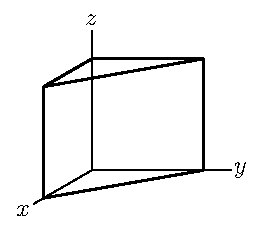
\includegraphics[scale=0.7,page=1]{fig/text.pdf} \\
    \includegraphics[scale=0.7,page=2]{fig/text.pdf} \\
    \includegraphics[scale=0.7,page=3]{fig/text.pdf} 
  \end{minipage}
  \begin{minipage}{0.25\textwidth}
    \includegraphics[scale=0.6,page=4]{fig/text.pdf} \\
    \includegraphics[scale=0.6,page=5]{fig/text.pdf}
  \end{minipage}
  \begin{minipage}{0.6\textwidth}
    \begin{align*}
      \int_E f(x, y, z)\,\text{d}V 
      &= \int_0^2\!\!\int_0^{4 - x}\!\!\int_0^{4 - x^2}\!\!f(x, y, z)\,\text{d}z\,\text{d}y\,\text{d}x \\
      &= \int_0^4\!\!\int_0^{\sqrt{4 - z}}\!\!\int_0^{4 - x}\!\!f(x, y, z)\,\text{d}y\,\text{d}x\,\text{d}z
    \end{align*}
  \end{minipage}
\end{sol}

\begin{ex}
  寫出 $\ds\int_0^2\!\int_0^{2 - y}\!\!\int_{0}^{\frac{2 - y}{2}}\!\!f(x, y, z)\,\text{d}x\,\text{d}z\,\text{d}y$ 依積分順序 $x\to y\to z$ 與 $y\to x\to z$ 之積分式.
\end{ex}

\begin{sol}
  \begin{minipage}{0.23\textwidth}
    \includegraphics[scale=0.62,page=7]{fig/text.pdf} \\
    \includegraphics[scale=0.62,page=8]{fig/text.pdf} \\
    \includegraphics[scale=0.62,page=10]{fig/text.pdf} 
  \end{minipage}
  \begin{minipage}{0.23\textwidth}
    \includegraphics[scale=0.62,page=9]{fig/text.pdf} \\
    \includegraphics[scale=0.62,page=11]{fig/text.pdf} \\
    \includegraphics[scale=0.62,page=12]{fig/text.pdf} 
  \end{minipage}
  \begin{minipage}{0.54\textwidth}
    \begin{align*}
      &\quad\;\int_0^2\!\!\int_0^{2 - y}\!\!\int_0^{\frac{2 - y}{2}}\!\!f(x, y, z)\,\text{d}x\,\text{d}z\,\text{d}y \\
      &= \int_0^2\!\!\int_0^{2 - z}\!\!\int_0^{\frac{2 - y}{2}}\!\!f(x, y, z)\,\text{d}x\,\text{d}y\,\text{d}z \\
      &= \int_0^2\!\!\int_0^{\frac{z}{2}}\!\!\int_0^{2 - z}\!\!f(x, y, z)\,\text{d}y\,\text{d}x\,\text{d}z \\
      &\quad+\int_0^2\!\!\int_{\frac{z}{2}}^{1}\!\!\int_0^{2 - 2x}\!\!f(x, y, z)\,\text{d}y\,\text{d}x\,\text{d}z
    \end{align*}
  \end{minipage}
\end{sol}

\begin{ex}
  若 $\ds\int_E f(x, y, z)\,\text{d}V = \int_0^1\!\int_{\sqrt{x}}^{1}\int_0^{1 - y}\!\!f(x, y, z)\,\text{d}z\,\text{d}y\,\text{d}x$, 寫出所有積分順序積分式.
\end{ex}

\begin{sol}
  \begin{minipage}{0.45\textwidth}
    
\includegraphics[scale=0.7,page=12]{fig/prob.pdf} \\
    
\includegraphics[scale=0.7,page=11]{fig/prob.pdf} \\ 
    
\includegraphics[scale=0.6,page=10]{fig/prob.pdf} 
  \end{minipage}
  \quad
  \begin{minipage}{0.55\textwidth}
    \begin{align*}
      &\;\quad\int_E f(x, y, z)\,\text{d}V & \\
      &= \int_0^1\!\int_{\sqrt{x}}^{1}\int_0^{1 - y}\!\!f(x, y, z)\,\text{d}z\,\text{d}y\,\text{d}x \\
      &= \int_0^1\!\int_{0}^{y^2}\!\!\!\int_0^{1 - y}\!\!f(x, y, z)\,\text{d}z\,\text{d}x\,\text{d}y \\
      &= \int_0^1\!\int_{0}^{1 - \sqrt{x}}\!\!\int_{\sqrt{x}}^{1 - z}\!\!f(x, y, z)\,\text{d}y\,\text{d}z\,\text{d}x \\
      &= \int_0^1\!\int_{0}^{(1 - z)^2}\!\!\!\int_{\sqrt{x}}^{1 - z}\!\!f(x, y, z)\,\text{d}y\,\text{d}x\,\text{d}z \\
      &= \int_0^1\!\int_{0}^{1 - y}\!\!\!\int_{0}^{y^2}\!\!f(x, y, z)\,\text{d}x\,\text{d}z\,\text{d}y \\
      &= \int_0^1\!\int_{0}^{1 - z}\!\!\!\int_0^{y^2}\!\!f(x, y, z)\,\text{d}x\,\text{d}y\,\text{d}z 
    \end{align*}
  \end{minipage}
\end{sol}

\begin{ex}
  若 $\ds\int_E f(x, y, z)\,\text{d}V = \int_{-1}^1\!\int_0^{1 - y^2}\!\!\int_0^{2 - y - z}\!\!f(x, y, z)\,\text{d}x\,\text{d}z\,\text{d}y$, 寫出依積分順序 $z\to x\to y$ 之積分式.
\end{ex}

\begin{sol}
  \begin{minipage}{0.25\textwidth}
    
\includegraphics[scale=0.62,page=2]{fig/prob.pdf} \\
    
\includegraphics[scale=0.56,page=3]{fig/prob.pdf} 
  \end{minipage}
  \begin{minipage}{0.25\textwidth}
    
\includegraphics[scale=0.68,page=4]{fig/prob.pdf} \\
    
\includegraphics[scale=0.68,page=5]{fig/prob.pdf} 
  \end{minipage}
  \quad
  \begin{minipage}{0.5\textwidth}
    \begin{align*}
      &\;\quad\int_E f(x, y, z)\,\text{d}V & \\
      &= \int_{-1}^1\int_0^{1 + y^2 - y}\!\!\int_0^{1 - y^2}\!\!f(x, y, z)\,\text{d}z\,\text{d}x\,\text{d}y \\
      &\quad + \int_{-1}^1\int_{1 + y^2 - y}^{2 - y}\int_0^{2 - x - y}\!\!f(x, y, z)\,\text{d}z\,\text{d}x\,\text{d}y 
    \end{align*}
  \end{minipage}
\end{sol}

\begin{ex}
  若 $E$ 為 $z = 2x$, $z = y^2$, $x = 3$ 圍成之區域, 寫出 $\ds\int_E f(x, y, z)\,\text{d}V$ 依積分順序 $z\to x\to y$, $x\to z\to y$, 與 $y\to x\to z$ 之積分式.
\end{ex}

\begin{sol}
  \begin{minipage}{0.6\textwidth}
    
\includegraphics[scale=0.82,page=23]{fig/prob.pdf} 
    
\includegraphics[scale=0.82,page=24]{fig/prob.pdf} 
    
\includegraphics[scale=0.82,page=25]{fig/prob.pdf} \\
    
\includegraphics[scale=0.88,page=26]{fig/prob.pdf} 
    
\includegraphics[scale=0.65,page=27]{fig/prob.pdf} 
    
\includegraphics[scale=0.7,page=28]{fig/prob.pdf} 
  \end{minipage}
  \begin{minipage}{0.4\textwidth}
    \begin{align*}
      &\quad\;\int_E f(x, y, z)\,\text{d}V \\
      &= \int_{-\sqrt{6}}^{\sqrt{6}}\int_{\frac{y^2}{2}}^{3}\!\int_{y^2}^{2x}\!\!f(x, y, z)\,\text{d}z\,\text{d}x\,\text{d}y \\
      &= \int_{-\sqrt{6}}^{\sqrt{6}}\int_{y^2}^{6}\!\!\int_{\frac{z}{2}}^3\!\!f(x, y, z)\,\text{d}x\,\text{d}z\,\text{d}y \\
      &= \int_0^6\!\!\int_{\frac{z}{2}}^{3}\!\!\int_{-\sqrt{z}}^{\sqrt{z}}\!\!f(x, y, z)\,\text{d}y\,\text{d}x\,\text{d}z
    \end{align*}
  \end{minipage}
\end{sol}

%\begin{ex}
%  若 $\ds\int_E f(x, y, z)\,\text{d}V = \int_0^1\!\int_0^{1 - \frac{x}{2}}\!\!\int_{0}^{4 - 2x - 4z}\!\!f(x, y, z)\,\text{d}y\,\text{d}z\,\text{d}x$, 寫出依積分順序 $z\to x\to y$ 之積分式.
%\end{ex}
%
%\begin{sol}
%  \begin{minipage}{0.28\textwidth}
%    
\includegraphics[scale=0.62,page=6]{fig/prob.pdf} \\
%    
\includegraphics[scale=0.62,page=7]{fig/prob.pdf} 
%  \end{minipage}
%  \begin{minipage}{0.28\textwidth}
%    
\includegraphics[scale=0.62,page=8]{fig/prob.pdf} \\
%    
\includegraphics[scale=0.62,page=9]{fig/prob.pdf} 
%  \end{minipage}
%  \quad
%  \begin{minipage}{0.44\textwidth}
%    \begin{align*}
%      &\;\quad\int_E f(x, y, z)\,\text{d}V & \\
%      &= \int_0^2\!\int_0^1\!\!\int_0^{\frac{4 - 2x - y}{2}}\!\!f(x, y, z)\,\text{d}z\,\text{d}x\,\text{d}y \\
%      &\quad + \int_2^4\!\int_0^{\frac{4 - y}{2}}\!\!\int_0^{\frac{4 - 2x - y}{2}}\!\!f(x, y, z)\,\text{d}z\,\text{d}x\,\text{d}y 
%    \end{align*}
%  \end{minipage}
%\end{sol}

\begin{ex}
  若 $E$ 為 $x^2 + y^2 = 1$, $z = y$, $z = -1$ 圍成之區域, 寫出 $\ds\int_E f(x, y, z)\,\text{d}V$ 依積分順序 $z\to x\to y$, $x\to y\to z$, 與 $y\to z\to x$ 之積分式.
\end{ex}

\begin{sol}
  \begin{minipage}{0.57\textwidth}
    
\includegraphics[scale=0.8,page=30]{fig/prob.pdf}\hspace{-8mm} 
    
\includegraphics[scale=0.75,page=31]{fig/prob.pdf} 
    
\includegraphics[scale=0.8,page=32]{fig/prob.pdf} \\ 
    
\includegraphics[scale=0.8,page=33]{fig/prob.pdf} 
  \end{minipage}
  \begin{minipage}{0.43\textwidth}
    \begin{align*}
      &\quad\;\int_E f(x, y, z)\,\text{d}V \\
      &= \int_{-1}^{1}\int_{-\sqrt{1 - y^2}}^{\sqrt{1 - y^2}}\!\int_{-1}^{y}\!f(x, y, z)\,\text{d}z\,\text{d}x\,\text{d}y \\
      &= \int_{-1}^{1}\int_{z}^{1}\!\!\int_{-\sqrt{1 - y^2}}^{\sqrt{1 - y^2}}\!f(x, y, z)\,\text{d}x\,\text{d}y\,\text{d}z \\
      &= \int_{-1}^{1}\int_{-1}^{-\sqrt{1 - x^2}}\!\!\!\!\int_{-\sqrt{1 - x^2}}^{\sqrt{1 - x^2}}\!f(x, y, z)\,\text{d}y\,\text{d}z\,\text{d}x \\
      &\quad + \int_{-1}^{1}\int_{-\sqrt{1 - x^2}}^{\sqrt{1 - x^2}}\!\int_{z}^{\sqrt{1 - x^2}}\!f(x, y, z)\,\text{d}y\,\text{d}z\,\text{d}x 
    \end{align*}
  \end{minipage}
\end{sol}

\begin{ex}
  若 $E$ 為 $z = x^2$, $y + z = 3$, $y = 0$, $y = 2$ 圍成之區域, 寫出 $\ds\int_E f(x, y, z)\,\text{d}V$ 依積分順序 $z\to x\to y$, $x\to y\to z$, 與 $y\to x\to z$ 之積分式.
\end{ex}

\begin{sol}
  \begin{minipage}{0.15\textwidth}
    
\includegraphics[scale=0.6,page=34]{fig/prob.pdf} \\
    
\includegraphics[scale=0.6,page=35]{fig/prob.pdf} \\ 
    
\includegraphics[scale=0.6,page=36]{fig/prob.pdf} 
  \end{minipage}
  \begin{minipage}{0.3\textwidth}
    
\includegraphics[scale=0.85,page=37]{fig/prob.pdf} \\
    \includegraphics[scale=0.85,page=38]{fig/prob.pdf} \\ 
  \end{minipage}
  \begin{minipage}{0.55\textwidth}
    \begin{align*}
      &\quad\;\int_E f(x, y, z)\,\text{d}V \\
      &= \int_{0}^{2}\!\int_{-\sqrt{3 - y}}^{\sqrt{3 - y}}\int_{3 - y}^{x^2}f(x, y, z)\,\text{d}z\,\text{d}x\,\text{d}y \\
      &= \int_{0}^{1}\!\int_{0}^{2}\!\int_{-\sqrt{z}}^{\sqrt{z}} f(x, y, z)\,\text{d}x\,\text{d}y\,\text{d}z \\
      &\quad + \int_{1}^{3}\!\!\int_{0}^{3 - z}\!\!\int_{-\sqrt{z}}^{\sqrt{z}}f(x, y, z)\,\text{d}x\,\text{d}y\,\text{d}z \\
      &= \int_{0}^{1}\!\int_{-\sqrt{z}}^{\sqrt{z}}\int_{0}^{2}\!f(x, y, z)\,\text{d}y\,\text{d}x\,\text{d}z \\
      &\quad + \int_{1}^{3}\!\int_{-\sqrt{z}}^{\sqrt{z}}\int_{0}^{3 - z}\!\!f(x, y, z)\,\text{d}y\,\text{d}x\,\text{d}z 
    \end{align*}
  \end{minipage}
\end{sol}

\begin{ex}
  寫出 $\ds\int_0^1\!\!\int_0^{1 - z}\!\!\!\int_0^{2}\!\!\,\text{d}x\,\text{d}y\,\text{d}z$ 所有積分順序積分式.
\end{ex}

\begin{sol}
  $\ds\int_0^1\!\!\int_0^{1 - z}\!\!\!\int_0^{2}\!\!\,\text{d}x\,\text{d}y\,\text{d}z = \int_0^1\!\!\int_0^{1 - y}\!\!\!\int_0^2\!\!\,\text{d}x\,\text{d}z\,\text{d}y = \int_0^2\!\!\int_0^1\!\!\int_0^{1 - y}\!\!\,\text{d}z\,\text{d}y\,\text{d}x = \int_0^1\!\!\int_0^2\!\!\int_0^{1 - y}\!\!\,\text{d}z\,\text{d}x\,\text{d}y = \int_0^2\!\!\int_0^{1}\!\!\!\int_0^{1 - z}\!\!\,\text{d}y\,\text{d}z\,\text{d}x \\= \int_0^1\!\!\int_0^2\!\!\!\int_0^{1 - z}\!\!\,\text{d}y\,\text{d}x\,\text{d}z = 1$.
\end{sol}

\begin{ex}
  若 $E$ 為以 $(0, 0, 0)$, $(1, 1, 0)$, $(0, 1, 0)$, $(0, 1, 1)$ 為頂點之四面體, 寫出 $\ds\int_E\text{d}V$ 所有積分順序積分式.
\end{ex}

\begin{sol}
  $E$ 之四面分別為 $z = 0$, $x = 0$, $y = 1$, $x - y + z = 0$ ($\ds\because(1, 1, 0)\times(0, 1, 1) = (1, -1, 1)$), 故 \\$\ds\int_E\text{d}V = \int_0^1\!\!\int_1^{x}\!\!\int_0^{y - x}\!\!\,\text{d}z\,\text{d}y\,\text{d}x = \int_0^1\!\!\int_0^{y}\!\!\int_0^{y - x}\!\!\,\text{d}z\,\text{d}x\,\text{d}y = \int_0^1\!\!\int_0^{1 - x}\!\!\!\int_{x + z}^1\!\!\,\text{d}y\,\text{d}z\,\text{d}x = \int_0^1\!\!\int_0^{1 - z}\!\!\!\int_{x + z}^1\!\!\,\text{d}y\,\text{d}x\,\text{d}z \\ = \int_0^1\!\!\int_z^{1}\!\!\int_0^{y - z}\!\!\,\text{d}x\,\text{d}y\,\text{d}z = \int_0^1\!\!\int_0^{y}\!\!\int_0^{y - z}\!\!\,\text{d}x\,\text{d}z\,\text{d}y = \frac{1}{6}$.
\end{sol}

\begin{ex}
  寫出 $\ds\int_0^1\!\!\int_y^{1}\!\!\int_0^{z}\!\!\,\text{d}x\,\text{d}z\,\text{d}y$ 所有積分順序積分式.
\end{ex}

\begin{sol}
  $\ds\int_0^1\!\!\int_y^{1}\!\!\int_0^{z}\!\!\,\text{d}x\,\text{d}z\,\text{d}y = \int_0^1\!\!\int_0^z\!\!\int_0^z\!\!\,\text{d}x\,\text{d}y\,\text{d}z = \int_0^1\!\!\int_x^1\!\!\int_y^1\!\!\,\text{d}z\,\text{d}y\,\text{d}x + \int_0^1\!\!\int_0^{x}\!\!\int_x^1\!\!\,\text{d}z\,\text{d}y\,\text{d}x \\= \int_0^1\!\!\int_0^{y}\!\!\int_y^1\!\!\,\text{d}z\,\text{d}x\,\text{d}y + \int_0^1\!\!\int_y^1\!\!\int_x^{1}\!\!\,\text{d}z\,\text{d}x\,\text{d}y = \int_0^1\!\!\int_x^{1}\!\!\!\int_0^z\!\!\,\text{d}y\,\text{d}z\,\text{d}x = \int_0^1\!\!\int_0^z\!\!\!\int_0^z\!\!\,\text{d}y\,\text{d}x\,\text{d}z = \frac{1}{3}$.
\end{sol}

\begin{ex}
  寫出 $\ds\int_0^1\!\!\int_0^{x^2}\!\!\!\int_0^{y}\!\!\,\text{d}z\,\text{d}y\,\text{d}x$ 所有積分順序積分式.
\end{ex}

\begin{sol}
  $\ds\int_0^1\!\!\int_0^{x^2}\!\!\!\int_0^{y}\!\!\,\text{d}z\,\text{d}y\,\text{d}x = \int_0^1\!\!\int_{\sqrt{y}}^1\int_0^{y}\!\!\,\text{d}z\,\text{d}x\,\text{d}y = \int_0^1\!\!\int_z^1\!\!\int_{\sqrt{y}}^1\!\!\,\text{d}x\,\text{d}y\,\text{d}z = \int_0^1\!\!\int_0^y\!\!\int_{\sqrt{y}}^1\!\!\,\text{d}x\,\text{d}z\,\text{d}y = \int_0^1\!\!\int_0^{x^2}\!\!\!\int_z^{x^2}\!\!\,\text{d}y\,\text{d}z\,\text{d}x \\= \int_0^1\!\!\int_{\sqrt{z}}^1\int_z^{x^2}\!\!\,\text{d}y\,\text{d}x\,\text{d}z = \frac{1}{10}$.
\end{sol}

\begin{ex}
  寫出 $\ds\int_0^1\!\!\int_y^{1}\!\!\!\int_0^{y}\!\!\,\text{d}z\,\text{d}x\,\text{d}y$ 所有積分順序積分式.
\end{ex}

\begin{sol}
  $\ds\int_0^1\!\!\int_y^{1}\!\!\int_0^{y}\!\!\,\text{d}z\,\text{d}x\,\text{d}y = \int_0^1\!\!\int_0^{x}\!\!\int_0^{y}\!\!\,\text{d}z\,\text{d}y\,\text{d}x = \int_0^1\!\!\int_z^1\!\!\int_{y}^1\!\!\,\text{d}x\,\text{d}y\,\text{d}z = \int_0^1\!\!\int_0^y\!\!\int_{y}^1\!\!\,\text{d}x\,\text{d}z\,\text{d}y = \int_0^1\!\!\int_0^{x}\!\!\int_z^{x}\!\!\,\text{d}y\,\text{d}z\,\text{d}x \\= \int_0^1\!\!\int_{z}^1\!\!\int_z^{x}\!\!\,\text{d}y\,\text{d}x\,\text{d}z = \frac{1}{6}$.
\end{sol}

\begin{ex}
  寫出 $\ds\int_0^1\!\!\int_{\!\!\sqrt{x}}^{1}\int_0^{1 - y}\!\!\,\text{d}z\,\text{d}y\,\text{d}x$ 所有積分順序積分式.
\end{ex}

\begin{sol}
  $\ds\int_0^1\!\!\int_{\!\!\sqrt{x}}^{1}\int_0^{1 - y}\!\!\,\text{d}z\,\text{d}y\,\text{d}x= \int_0^1\!\!\int_0^{y^2}\!\!\!\!\int_0^{1 - y}\!\!\,\text{d}z\,\text{d}x\,\text{d}y = \int_0^1\!\!\int_0^{1 - z}\!\!\!\!\int_{0}^{y^2}\!\!\,\text{d}x\,\text{d}y\,\text{d}z = \int_0^1\!\!\int_0^{1 - y}\!\!\!\!\int_{0}^{y^2}\!\!\,\text{d}x\,\text{d}z\,\text{d}y \\= \int_0^1\!\!\int_0^{1 - \sqrt{x}}\!\!\!\!\int_{\sqrt{x}}^{1 - z}\!\!\,\text{d}y\,\text{d}z\,\text{d}x = \int_0^1\!\!\int_{0}^{(1 - z)^2}\!\!\!\!\!\int_{\sqrt{x}}^{1 - z}\!\!\,\text{d}y\,\text{d}x\,\text{d}z = \frac{1}{12}$.
\end{sol}

\begin{ex}
  寫出 $\ds\int_0^1\!\!\int_0^{1 - x^2}\!\!\!\!\int_0^{1 - x}\!\!\,\text{d}y\,\text{d}z\,\text{d}x$ 所有積分順序積分式.
\end{ex}

\begin{sol}
  $\ds\int_0^1\!\!\int_0^{1 - x^2}\!\!\!\!\int_0^{1 - x}\!\!\,\text{d}y\,\text{d}z\,\text{d}x = \int_0^1\!\!\int_0^{\sqrt{1 - z}}\!\!\!\!\int_0^{1 - x}\!\!\,\text{d}y\,\text{d}x\,\text{d}z = \int_0^1\!\!\int_0^{1 - x}\!\!\!\!\int_0^{1 - x^2}\!\!\,\text{d}z\,\text{d}y\,\text{d}x = \int_0^1\!\!\int_0^{1 - y}\!\!\!\!\int_0^{1 - x^2}\!\!\,\text{d}z\,\text{d}x\,\text{d}y = \int_0^1\!\!\int_0^{1 - \sqrt{1 - z}}\!\!\!\!\int_0^{\sqrt{1 - z}}\!\!\,\text{d}x\,\text{d}y\,\text{d}z + \int_0^1\!\!\int_{1 - \sqrt{1 - z}}^1\!\int_0^{1 - y}\!\!\,\text{d}x\,\text{d}y\,\text{d}z = \int_0^1\!\!\int_{2y - y^2}^1\!\int_0^{\sqrt{1 - z}}\!\!\,\text{d}x\,\text{d}z\,\text{d}y + \int_0^1\!\!\int_0^{2y - y^2}\!\!\!\!\!\int_0^{1 - y}\!\!\,\text{d}x\,\text{d}z\,\text{d}y = \frac{5}{12}$.
\end{sol}

\begin{ex}
  寫出 $\ds\int_{-1}^1\!\int_{-\sqrt{1 - x^2}}^{\sqrt{1 - x^2}}\!\int_{\sqrt{x^2 + y^2}}^1\!\!\,\text{d}z\,\text{d}y\,\text{d}x$ 所有積分順序積分式.
\end{ex}

\begin{sol}
  $\ds\int_{-1}^1\!\int_{-\sqrt{1 - x^2}}^{\sqrt{1 - x^2}}\!\int_{\sqrt{x^2 + y^2}}^1\!\!\,\text{d}z\,\text{d}y\,\text{d}x = \int_{-1}^1\!\int_{-\sqrt{1 - y^2}}^{\sqrt{1 - y^2}}\!\int_{\sqrt{x^2 + y^2}}^1\!\!\,\text{d}z\,\text{d}x\,\text{d}y\\ = \int_0^1\!\!\int_{-z}^{z}\!\int_{-\sqrt{z^2 - x^2}}^{\sqrt{z^2 - x^2}}\!\!\,\text{d}y\,\text{d}x\,\text{d}z = \int_{-1}^0\!\int_{-x}^{1}\!\int_{-\sqrt{z^2 - x^2}}^{\sqrt{z^2 - x^2}}\!\!\,\text{d}y\,\text{d}z\,\text{d}x + \int_0^1\!\!\int_{x}^{1}\!\!\int_{-\sqrt{z^2 - x^2}}^{\sqrt{z^2 - x^2}}\!\!\,\text{d}y\,\text{d}z\,\text{d}x \\= \int_0^1\!\!\int_{-z}^{z}\!\int_{-\sqrt{z^2 - y^2}}^{\sqrt{z^2 - y^2}}\!\!\,\text{d}x\,\text{d}y\,\text{d}z = \int_{-1}^0\!\int_{-y}^1\!\int_{-\sqrt{z^2 - y^2}}^{\sqrt{z^2 - y^2}}\!\!\,\text{d}x\,\text{d}z\,\text{d}y + \int_0^1\!\int_{y}^1\!\!\int_{-\sqrt{z^2 - y^2}}^{\sqrt{z^2 - y^2}}\!\!\,\text{d}x\,\text{d}z\,\text{d}y = \frac{\pi}{3}$.
\end{sol}

\begin{ex}
  證明 $\ds\int_0^{x}\!\int_0^{y}\!\int_0^{z}\!f(t)\,\text{d}t\,\text{d}z\,\text{d}y = \frac{1}{2}\int_0^{x}(x - t)^2f(t)\,\text{d}t$.
\end{ex}

\begin{sol}
  建立 $(t, z, y)$ 座標系, 其相對位置如 $(x, y, z)$; $\ds\int_0^{x}\!\int_0^{y}\!\int_0^{z}\!f(t)\,\text{d}t\,\text{d}z\,\text{d}y = \int_0^{x}\!\int_t^{x}\!\int_{t}^{y}\!f(t)\,\text{d}z\,\text{d}y\,\text{d}t \\= \int_0^{x}\!\int_t^{x}\!(y - t)\,f(t)\,\text{d}y\,\text{d}t = \int_0^{x}\Big(\frac{x^2 - t^2}{2} f(t) - (x - t)\,t\,f(t)\Big)\,\text{d}t = \frac{1}{2}\int_0^x(x - t)^2 f(t)\,\text{d}t$. 
\end{sol}

}{}

\subsection*{變數變換}

\subsubsection*{柱面座標}
\begin{minipage}{0.25\textwidth}
  \includegraphics[scale=1,page=13]{fig/text.pdf} \\
\end{minipage}
\begin{minipage}{0.75\textwidth}
  \begin{align*}
    \begin{cases}
      x = r\cos\theta \\
      y = r\sin\theta \\
      z = z
    \end{cases} \ifff \quad
    \begin{cases}
      r = \sqrt{x^2 + y^2}\\
      \theta = \tan^{-1}\frac{y}{x} \\
      z = z 
    \end{cases}
  \end{align*}
  \begin{align*}
    \text{Jacobian } J_{\vx}(\vu) = \frac{\partial\vx}{\partial\vu}(\vu) = \begin{vmatrix}\frac{\partial x}{\partial r} & \frac{\partial x}{\partial\theta} & \frac{\partial x}{\partial z} \\ \frac{\partial y}{\partial r} & \frac{\partial y}{\partial\theta} & \frac{\partial y}{\partial z} \\ \frac{\partial z}{\partial r} & \frac{\partial z}{\partial\theta} & \frac{\partial z}{\partial z} \end{vmatrix} = \begin{vmatrix}\cos\theta & -r\sin\theta & 0 \\ \sin\theta & r\cos\theta & 0 \\ 0 & 0 & 1\end{vmatrix} = r
  \end{align*}
\end{minipage}

\subsubsection*{球面座標}
\begin{minipage}{0.3\textwidth}
  \includegraphics[scale=0.9,page=14]{fig/text.pdf} \\
\end{minipage}
\begin{minipage}{0.7\textwidth}
  \begin{align*}
    \begin{cases}
      x = \rho\sin\varphi\cos\theta \\
      y = \rho\sin\varphi\sin\theta \\
      z = \rho\cos\varphi 
    \end{cases} \ifff \quad
    \begin{cases}
      \rho = \sqrt{x^2 + y^2 + z^2}\\
      \theta = \tan^{-1}\frac{y}{x} \\
      \varphi = \tan^{-1}\frac{\sqrt{x^2 + y^2}}{z} 
    \end{cases}
  \end{align*}
  \begin{align*}
    \text{Jacobian } J_{\vx}(\vu) &= \frac{\partial\vx}{\partial\vu}(\vu) = \begin{vmatrix}\frac{\partial x}{\partial\rho} & \frac{\partial x}{\partial\theta}  & \frac{\partial x}{\partial\varphi} \\ \frac{\partial y}{\partial\rho} & \frac{\partial y}{\partial\theta} & \frac{\partial y}{\partial\varphi}\\ \frac{\partial z}{\partial\rho} & \frac{\partial z}{\partial\theta} & \frac{\partial z}{\partial\varphi}\end{vmatrix} \\ &= \begin{vmatrix}\sin\varphi\cos\theta & -\rho\sin\varphi\sin\theta & \rho\cos\varphi\cos\theta \\ \sin\varphi\sin\theta & \rho\sin\varphi\cos\theta & \rho\cos\varphi\sin\theta\\ \cos\varphi & 0 & -\rho\sin\varphi\end{vmatrix} = -\rho^2\sin\varphi
  \end{align*}
\end{minipage}

\begin{ex}
  半徑為 $a$ 之球中心對稱鑽半徑為 $b$ 之圓孔, $a > b > 0$, 求球剩下的體積.
\end{ex}

\begin{sol}
  \begin{minipage}{0.25\textwidth}
    \includegraphics[scale=0.62,page=17]{fig/text.pdf} 
  \end{minipage}
  \begin{minipage}{0.75\textwidth}
    %\begin{align*}
    %  \text{(體積)} &= 8\cdot\int_0^{\frac{\pi}{2}}\!\!\int_b^a\!\int_0^{\sqrt{a^2 - r^2}}\!r\,\text{d}z\,\text{d}r\,\text{d}\theta \\
    %  &= 4\pi\cdot\int_b^a r\sqrt{a^2 - r^2}\,\text{d}r \\
    %  &= 4\pi\cdot\Big(\frac{-1}{3}(a^2 - r^2)^{\frac{3}{2}}\,\Big|_b^a\Big) = \frac{4\pi}{3}(a^2 - b^2)^{\frac{3}{2}}
    %\end{align*}
    \begin{itemize}
      \item 柱面座標: $\ds\int_E\text{d}V = 8\int_0^{\frac{\pi}{2}}\!\!\int_b^a\!\int_0^{\sqrt{a^2 - r^2}}\!r\,\text{d}z\,\text{d}r\,\text{d}\theta = \frac{4\pi}{3}(a^2 - b^2)^{\frac{3}{2}}$ 
      \item 球面座標: $\ds\int_E\text{d}V = 2\int_{\sin^{-1}\!\!\frac{b}{a}}^{\frac{\pi}{2}}\!\int_0^{2\pi}\!\!\!\int_{\frac{b}{\sin\varphi}}^{a}\rho^2\sin\varphi\,\text{d}\rho\,\text{d}\theta\,\text{d}\varphi = \frac{4\pi}{3}(a^2 - b^2)^{\frac{3}{2}}$
    \end{itemize}
  \end{minipage}
\end{sol}

\begin{ex}
  若 $E$ 為 $x^2 + y^2 \leqslant z^2$, $x^2 + y^2 + z^2 \leqslant 1$ 與 $z\geqslant 0$ 圍成之區域, 求 $\ds\int_E \sqrt{x^2 + y^2 + z^2}\,\text{d}V$.
\end{ex}

\begin{sol}
  \begin{minipage}{0.4\textwidth}
    \includegraphics[scale=0.7,page=64]{fig/prob.pdf} \\ 
  \end{minipage}
  \begin{minipage}{0.6\textwidth}
    \begin{itemize}
      \item 柱面座標: $\ds\int_E\sqrt{x^2 + y^2 + z^2}\,\text{d}V \\= \int_0^{2\pi}\!\!\!\int_0^{\frac{1}{\sqrt{2}}}\!\!\int_{r}^{\sqrt{1 - r^2}}\!\!\!\sqrt{r^2 + z^2}\cdot r\,\text{d}z\,\text{d}r\,\text{d}\theta$ 
      \item 球面座標: $\ds\int_E\sqrt{x^2 + y^2 + z^2}\,\text{d}V \\= \int_0^{\frac{\pi}{4}}\!\!\!\int_0^{2\pi}\!\!\!\int_0^{1}\rho\cdot\rho^2\sin\varphi\,\text{d}\rho\,\text{d}\theta\,\text{d}\varphi = \frac{\pi}{2}\,\Big(1 - \frac{1}{\sqrt{2}}\Big)$
    \end{itemize}
  \end{minipage}
\end{sol}

\begin{ex}
  若 $E$ 為 $0\leqslant z \leqslant\sqrt{x^2 + y^2}$ 與 $x^2 + y^2 \leqslant 1$ 圍成之區域, 求 $\ds\int_E z\sqrt{x^2 + y^2 + z^2}\,\text{d}V$.
\end{ex}

\begin{sol}
  \begin{minipage}{0.22\textwidth}
    \includegraphics[scale=0.85,page=73]{fig/prob.pdf} \\ 
  \end{minipage}
  \begin{minipage}{0.78\textwidth}
    \begin{itemize}
      \item 柱面座標: $\ds\int_E z\sqrt{x^2 + y^2 + z^2}\,\text{d}V$ $=$ $\ds\int_0^{2\pi}\!\!\!\int_0^1\!\!\!\int_{0}^{r}\!z\sqrt{r^2 + z^2}\cdot r\,\text{d}z\,\text{d}r\,\text{d}\theta$ \\$=$ $\ds 2\pi\,\int_0^1\!\frac{r}{3}(r^2 + z^2)^{\frac{3}{2}}\,\Big|_{z = 0}^{z = r}\,\text{d}r = \frac{2\pi}{3}\int_0^1 r\cdot(2^{\frac{3}{2}} - 1)\,r^3\,\text{d}r = \frac{2\pi\,(2^{\frac{3}{2}} - 1)}{15}$ 
      \item 球面座標: $\ds\int_E z\sqrt{x^2 + y^2 + z^2}\,\text{d}V = \int_{\frac{\pi}{4}}^{\frac{\pi}{2}}\!\!\!\int_0^{2\pi}\!\!\!\int_0^{\frac{1}{\sin\varphi}}\!\!\rho\cos\varphi\cdot\rho\cdot\rho^2\sin\varphi\,\text{d}\rho\,\text{d}\theta\,\text{d}\varphi$
    \end{itemize}
  \end{minipage}
\end{sol}

\begin{ex}
  若 $E$ 為 $z = x^2 + y^2$ 與 $z \leqslant\sqrt{x^2 + y^2}$ 圍成之區域, 求 $\ds\int_E z\,(x^2 + y^2 + z^2)\,\text{d}V$.
\end{ex}

\begin{sol}
  \begin{minipage}{0.22\textwidth}
    \includegraphics[scale=0.95,page=76]{fig/prob.pdf} \\ 
  \end{minipage}
  \begin{minipage}{0.78\textwidth}
    \begin{itemize}
      \item 柱面座標: $\ds\int_E z\,(x^2 + y^2 + z^2)\,\text{d}V$ $=$ $\ds\int_0^{2\pi}\!\!\!\int_0^1\!\!\int_{r^2}^{r}\!z\,(r^2 + z^2)\cdot r\,\text{d}z\,\text{d}r\,\text{d}\theta$ \\$=$ $\ds 2\pi\int_0^1\!\!\int_{r^2}^{r}(r^3z + rz^3)\,\text{d}z\,\text{d}r$ $=$ $\ds 2\pi\int_0^1\Big(\frac{r^3}{2}(r^2 - r^4) + \frac{r}{4}(r^4 - r^8)\Big)\,\text{d}r = \frac{3\pi}{40}$ 
      \item 球面座標: $\ds z = x^2 + y^2 \ie \rho\cos\varphi = \rho^2\sin^2\varphi \ie \rho = \frac{\cos\varphi}{\sin^2\varphi}$; \\$\ds z = \sqrt{x^2 + y^2} \ie \rho\cos\varphi = \rho\sin\varphi \ie \tan\varphi = 1$; \\$\ds\int_E z\,(x^2 + y^2 + z^2)\,\text{d}V = \int_{\frac{\pi}{4}}^{\frac{\pi}{2}}\!\!\!\int_0^{2\pi}\!\!\!\int_0^{\frac{\cos\varphi}{\sin^2\varphi}}\!\!\rho\cos\varphi\cdot\rho^2\cdot\rho^2\sin\varphi\,\text{d}\rho\,\text{d}\theta\,\text{d}\varphi$
    \end{itemize}
  \end{minipage}
\end{sol}

\begin{ex}
  若 $E$ 為 $y = x^2 + z^2$ 與 $y = 4$ 圍成之區域, 求 $\ds\int_E \sqrt{x^2 + z^2}\,\text{d}V$.
\end{ex}

\begin{sol}
  令 $\ds\begin{cases}x = r\cos\theta \\ z = r\sin\theta \end{cases}\!\!\!\!\!$, 投影之 $\Omega$ 為 $x^2 + z^2 \leqslant 4$, 則 $\ds\int_E\sqrt{x^2 + z^2}\,\text{d}V = \int_\Omega\int_{x^2 + z^2}^4\sqrt{x^2 + z^2}\,\text{d}y\,\text{d}A \\= \int_\Omega(4 - (x^2 + z^2))\,\sqrt{x^2 + z^2}\,\text{d}A = \int_0^{2\pi}\!\!\!\int_0^2(4 - r^2)\,r\cdot r\,\text{d}r\,\text{d}\theta = 2\pi\int_0^2(4r^2 - r^4)\,\text{d}r = 2\pi\cdot\Big(\frac{4\cdot2^3}{3} - \frac{2^5}{5}\Big) = \frac{128\pi}{15}$.
\end{sol}

\begin{ex}
  若 $E = \{(x,\,y,\,z)\,|\, x^2 + y^2 + (z - 1)^2 \leqslant 1\}$, 求 $\ds\int_E (x^2 + y^2 + z^2)^{\frac{5}{2}}\,\text{d}V$.
\end{ex}

\begin{sol}
  代入球面座標於 $\ds x^2 + y^2 + (z - 1)^2 \leqslant 1\ie (\rho\sin\varphi\cos\theta)^2 + (\rho\sin\varphi\sin\theta)^2 + (\rho\cos\varphi - 1)^2\leqslant 1 \ie \rho^2\sin^2\varphi + \rho^2\cos^2\varphi - 2\rho\cos\varphi + 1\leqslant 1 \ie \rho^2\leqslant 2\rho\cos\varphi \ie \rho\leqslant 2\cos\varphi$, 故 $\ds\int_E (x^2 + y^2 + z^2)^{\frac{5}{2}}\,\text{d}V = \int_0^{\frac{\pi}{2}}\!\!\int_0^{2\pi}\!\!\!\int_0^{2\cos\varphi}\!\!\rho^5\cdot\rho^2\sin\varphi\,\text{d}\rho\,\text{d}\theta\,\text{d}\varphi = 2\pi\int_0^{\frac{\pi}{2}}\!\frac{(2\cos\varphi)^8}{8}\sin\varphi\,\text{d}\varphi = \frac{64\pi}{9}(-\cos^9\varphi)\,\Big|_0^{\frac{\pi}{2}} = \frac{64\pi}{9}$.
\end{sol}

\begin{ex}
  若 $E$ 為 $z = \sqrt{x^2 + y^2}$ 與 $x^2 + y^2 + (z - 1)^2 = 1$ 於第一卦限圍成之區域, 求其體積.
\end{ex}

\begin{sol}
  \begin{minipage}{0.4\textwidth}
    \includegraphics[scale=0.7,page=77]{fig/prob.pdf} \\ 
  \end{minipage}
  \begin{minipage}{0.6\textwidth}
    \begin{itemize}
      \item 柱面座標: $\ds\int_E\text{d}V = \int_0^{\frac{\pi}{2}}\!\!\!\int_0^1\!\!\int_{r}^{1 + \sqrt{1 - r^2}}\!\!\!r\,\text{d}z\,\text{d}r\,\text{d}\theta = \frac{\pi}{4}$ 
      \item 球面座標: $\ds\int_E\text{d}V = \int_0^{\frac{\pi}{4}}\!\!\!\int_0^{\frac{\pi}{2}}\!\!\!\int_0^{2\cos\varphi}\!\!\!\rho^2\sin\varphi\,\text{d}\rho\,\text{d}\theta\,\text{d}\varphi = \frac{\pi}{4}$
    \end{itemize}
  \end{minipage}
\end{sol}

\section*{7.3 綜合問題}

\begin{thm}[積分下取微分]
  若 $f(x, y)$ 與 $\ds\frac{\partial f}{\partial y}(x, y)$ 在 $[a, b]\times[c, d]$ 連續, 設 $\ds F(y) = \int_{a}^{b}f(x, y)\,\mathrm{d}x$, 則 $\ds F'(y) = \int_{a}^{b}\frac{\partial f}{\partial y}(x, y)\,\mathrm{d}x$.
\end{thm}

\begin{prf}
  若 $y_0\in(c, d)$ 且 $y\ne y_0$, $\ds\frac{F(y) - F(y_0)}{y - y_0} = \int_a^b\frac{f(x, y) - f(x, y_0)}{y - y_0}\,\mathrm{d}x\to\int_a^b\frac{\partial f}{\partial y}(x, y_0)\,\mathrm{d}x$.
\end{prf}

%\begin{thm}[積分下取微分]
%  若 $f(x, y)$ 與 $\ds\frac{\partial f}{\partial y}(x, y)$ 在 $[a, b]\times[c, d]$ 連續, $p$, $q$ 在 $[c, d]$ 可微, 且 $\forall\,y\in[c, d]$, $p(y),\,q(y)\in[a, b]$; 設 $\ds F(y) = \int_{p(y)}^{q(y)}f(x, y)\,\mathrm{d}x$, 則 $\ds F'(y) = \int_{p(y)}^{q(y)}\frac{\partial f}{\partial y}(x, y)\,\mathrm{d}x + f(q(y), y)\,q'(y) - f(p(y), y)\,p'(y)$.
%\end{thm}
%
%\begin{prf}
%  令 $\ds G(x_1, x_2, x_3) = \int_{x_1}^{x_2}f(t, x_3)\,\mathrm{d}t$ $\forall\,x_1,\,x_2\in[a, b]$, $x_3\in[c, d]$, 則 $F(y) = G(p(y), q(y), y)$. 由鏈鎖律 $\ds F'(y) = G_1(p(y), q(y), y)\,p'(y) + G_2(p(y), q(y), y)\,q'(y) + G_3(p(y), q(y), y)$. 微積分基本定理結論 $G_1(x_1, x_2, x_3) = -f(x_1, x_3)$, $G_2(x_1, x_2, x_3) = f(x_2, x_3)$, 由上定理 $\ds G_3(x_1, x_2, x_3) = \int_{x_1}^{x_2}\frac{\partial f}{\partial y}(t, x_3)\,\mathrm{d}t$; 代回得證.
%\end{prf}

\begin{ex}
  證明 $\ds\int_0^\infty e^{-x^2}\,\mathrm{d}x = \frac{\sqrt{\pi}}{2}$.
\end{ex}

\begin{prf}
  令 $\ds F(t) = \int_0^\infty\!\frac{e^{-t^2(1 + x^2)}}{1 + x^2}\,\mathrm{d}x$, $t\geqslant 0$; $F(\infty) = 0$, $\ds F(0) = \int_0^\infty\!\!\frac{\mathrm{d}x}{1 + x^2} = \tan^{-1}x\,\Big|_0^\infty = \tan^{-1}\infty - \tan^{-1}0 = \frac{\pi}{2}$. 則 $\ds F'(t) = \int_0^\infty\!\frac{-2\,t\,(1 + x^2)\,e^{-t^2(1 + x^2)}}{1 + x^2}\,\mathrm{d}x = \underbrace{-2\,t\,e^{-t^2}\!\!\int_0^\infty\!e^{-t^2x^2}\,\mathrm{d}x}_{\text{令}\;u\,=\,t\,x,\;\text{則}\;\mathrm{d}u\,=\,t\,\mathrm{d}x} = -2\,e^{-t^2}\!\!\underbrace{\int_0^\infty\!e^{-u^2}\,\mathrm{d}u}_{=\,I} = -2\,e^{-t^2} I$ $\ie$ $\ds\int_0^b F'(t)\,\mathrm{d}t = -2 I\int_0^b\!e^{-t^2}\,\mathrm{d}t$ $\ie$ $\ds F(b) - F(0) = -2 I\int_0^b\!e^{-t^2}\,\mathrm{d}t$. 令 $b\to\infty$, 則 $\ds F(\infty) - F(0) = -2 I^2$ $\ie$ $\ds 0 - \frac{\pi}{2} = -2 I^2$ $\ie$ $\ds I = \frac{\sqrt{\pi}}{2}$.
\end{prf}

\begin{ex} 若 $a > 0$, 求
  \begin{multicols}{3}
    \begin{enumerate}
      \item $\ds\int_{-\infty}^\infty x^2 e^{-ax^2}\,\text{d}x$. 
      \item $\ds\int_{-\infty}^\infty x^4 e^{-ax^2}\,\text{d}x$.
      \item $\ds\int_{-\infty}^\infty x^6 e^{-ax^2}\,\text{d}x$.
    \end{enumerate}
  \end{multicols}
\end{ex}

\begin{sol} 已知 $\ds F(a) = \int_{-\infty}^\infty e^{-ax^2}\,\mathrm{d}x = \frac{\sqrt{\pi}}{\sqrt{a}} = \sqrt{\pi}\,a^{-\frac{1}{2}}$, 則
  \begin{enumerate}\setlength{\itemsep}{0pt}
    \item $\ds F'(a) = \frac{\mathrm{d}}{\mathrm{d}a}(\sqrt{\pi}\,a^{-\frac{1}{2}}) = \sqrt{\pi}\cdot\frac{-1}{2}\,a^{-\frac{3}{2}} = -\int_{-\infty}^\infty x^2 e^{-ax^2}\,\text{d}x$ $\ie$ $\ds\int_{-\infty}^\infty x^2 e^{-ax^2}\,\text{d}x = \frac{\sqrt{\pi}}{2\,a^{\frac{3}{2}}}$.
    \item $\ds F''(a) = \frac{\mathrm{d}^2}{\mathrm{d}a^2}(\sqrt{\pi}\,a^{-\frac{1}{2}}) = \sqrt{\pi}\cdot\frac{3}{4}\,a^{-\frac{5}{2}} = \int_{-\infty}^\infty x^4 e^{-ax^2}\,\text{d}x$ $\ie$ $\ds\int_{-\infty}^\infty x^4 e^{-ax^2}\,\text{d}x = \frac{3\sqrt{\pi}}{4\,a^{\frac{5}{2}}}$.
    \item $\ds F'''(a) = \frac{\mathrm{d}^3}{\mathrm{d}a^3}(\sqrt{\pi}\,a^{-\frac{1}{2}}) = \sqrt{\pi}\cdot\frac{-15}{8}a^{-\frac{7}{2}} = -\int_{-\infty}^\infty x^6 e^{-ax^2}\,\text{d}x$ $\ie$ $\ds\int_{-\infty}^\infty x^6 e^{-ax^2}\,\text{d}x = \frac{15\sqrt{\pi}}{8\,a^{\frac{7}{2}}}$.
  \end{enumerate}
\end{sol}

\begin{ex}
  證明 $\ds\int_0^\infty\!\!e^{-tx}\,\frac{\sin x}{x}\,\mathrm{d}x = \frac{\pi}{2} - \tan^{-1}t$, $\forall\,t > 0$.
\end{ex}

\begin{prf}
  令 $\ds F(t) = \int_0^\infty\!\!e^{-tx}\,\frac{\sin x}{x}\,\mathrm{d}x$, 則 $\ds F'(t) = -\int_0^\infty\!\!e^{-tx}\sin x\,\mathrm{d}x = -\frac{e^{-tx}(-t\sin x - \cos x)}{1 + t^2}\,\Big|_{x = 0}^{x = \infty} = -\frac{1}{1 + t^2}$ $\ie$ $\ds F(t) = -\tan^{-1}t + c$. 令 $t\to\infty$, $\ds F(\infty) = 0 = -\tan^{-1}\infty + c = -\frac{\pi}{2} + c$ $\ie$ $\ds c = \frac{\pi}{2}$.  
\end{prf}

\begin{ex}
  若 $a > 0$, 求 $\ds\int_0^\infty\!\!\frac{\mathrm{d}x}{(x^2 + a^2)^2}$, $\ds\int_0^\infty\!\!\frac{\mathrm{d}x}{(x^2 + a^2)^3}$ 並推導 $\ds\int_0^\infty\!\!\frac{\mathrm{d}x}{(x^2 + a^2)^n}$, $n\in\mathbb{N}$.
\end{ex}

\begin{sol}
  由 $\ds F(a) = \int_0^\infty\!\!\frac{\mathrm{d}x}{x^2 + a^2} = \frac{\pi}{2a} = \frac{\pi}{2}\,a^{-1}$, $\ds F'(a) = \frac{\mathrm{d}}{\mathrm{d}a}\Big(\frac{\pi}{2}\,a^{-1}\Big) = \frac{\pi}{2}(-1)\,a^{-2} = (-1)2a\int_0^\infty\!\!\frac{\mathrm{d}x}{(x^2 + a^2)^2}$ $\ie$ $\ds\int_0^\infty\!\!\frac{\mathrm{d}x}{(x^2 + a^2)^2} = \frac{\pi}{4\,a^3}$; 等式兩邊再對 $a$ 微分 $\ie$ $\ds(-2)(2a)\int_0^\infty\!\!\frac{\mathrm{d}x}{(x^2 + a^2)^3} = (-3)\frac{\pi}{4\,a^4}$ $\ie$ $\ds\int_0^\infty\!\!\frac{\mathrm{d}x}{(x^2 + a^2)^3} = \frac{3\,\pi}{16\,a^5}$. 由數學歸納法可得 $\ds\int_0^\infty\!\!\frac{\mathrm{d}x}{(x^2 + a^2)^n} = \frac{\pi}{(2a)^{2n - 1}}\binom{2(n - 1)}{n - 1}$, $n\in\mathbb{N}$.
\end{sol}

\begin{ex}
  證明 $\ds\int_0^\infty\!\!e^{-x^2}\!\cos tx\,\mathrm{d}x = \frac{\sqrt{\pi}}{2}\,e^{\frac{-t^2}{4}}$, $\forall\,t\in\mathbb{R}$.
\end{ex}

\begin{prf}
  令 $\ds F(t) = \int_0^\infty\!\!e^{-x^2}\!\cos tx\,\mathrm{d}x$, 則 $\ds F'(t) = -\int_0^\infty\!\!e^{-x^2}x\sin tx\,\mathrm{d}x$. 令 $\ds u = \frac{1}{2}\sin tx$, 則 $\ds\mathrm{d}u = \frac{t}{2}\cos tx$; 令 $\ds\mathrm{d}v = -2xe^{-x^2}\,\mathrm{d}x$, 則 $\ds v = e^{-x^2}$. 故 $\ds F'(t) = -\int_0^\infty\!\!e^{-x^2}x\sin tx\,\mathrm{d}x = \frac{1}{2}\sin tx\cdot e^{-x^2}\,\Big|_{x = 0}^{x = \infty} - \int_0^\infty\!\!e^{-x^2}\cdot\frac{t}{2}\cos tx\,\mathrm{d}x = -\frac{t}{2}F(t)$, 故 $\ds F(t) = c\,e^{\frac{-t^2}{4}}$; 又 $\ds F(0) = \frac{\sqrt{\pi}}{2} = c\cdot e^0 = c$.
\end{prf}

\begin{ex}
  已知 $\forall\;0 < \alpha < 1$, $\ds\int_0^\infty\!\frac{x^{\alpha - 1}}{1 + x}\,\text{d}x = \frac{\pi}{\sin\alpha\pi}$, 證明 $\ds\Gamma(\alpha)\,\Gamma(1 - \alpha) = \frac{\pi}{\sin\alpha\pi}$.
\end{ex}

\begin{sol}
  $\ds\Gamma(\alpha)\,\Gamma(1 - \alpha) = \int_0^\infty\!\!e^{-t}t^{\alpha - 1}\,\text{d}t\int_0^\infty\!\!e^{-s}s^{-\alpha}\,\text{d}s = \int_0^\infty\!\!\!\int_0^\infty\!\!e^{-(t + s)}t^{\alpha - 1}s^{-\alpha}\,\text{d}s\,\text{d}t$. 令 $\ds\begin{cases}u = s + t \\ v = \frac{t}{s}\end{cases}\!\!\!\!\!$, 則 $\ds\begin{cases}s = \frac{u}{1 + v}\\ t = \frac{uv}{1 + v}\end{cases}\!\!\!\!\!$; Jacobian $\ds J_{\vx}(\vu) = \frac{\partial\vx}{\partial\vu}(\vu) = \begin{vmatrix}\frac{\partial s}{\partial u} & \frac{\partial s}{\partial v} \\ \frac{\partial t}{\partial u}& \frac{\partial t}{\partial v}\end{vmatrix} = \begin{vmatrix}\frac{1}{1 + v} & \frac{-u}{(1 + v)^2} \\ \frac{v}{1 + v} & \frac{u}{(1 + v)^2}\end{vmatrix} = \frac{u}{(1 + v)^2}$. 變數變換 $(s,\,t)\to(u,\,v)$ 後積分範圍仍為 $0< u < \infty,\;0 < v < \infty$, 故 $\ds\int_0^\infty\!\!\!\int_0^\infty e^{-(t + s)}t^{\alpha - 1}s^{-\alpha}\,\text{d}s\,\text{d}t = \int_0^\infty\!\!\!\int_0^\infty e^{-(t + s)}\Big(\frac{t}{s}\Big)^{\alpha}t^{-1}\,\text{d}s\,\text{d}t = \int_0^\infty\!\!\!\int_0^\infty e^{-u}v^{\alpha}\frac{1 + v}{u v}\frac{u}{(1 + v)^2}\,\text{d}u\,\text{d}v = \int_0^\infty\!\!\!\int_0^\infty\!\! e^{-u}\frac{v^{\alpha - 1}}{1 + v}\,\text{d}u\,\text{d}v = \int_0^\infty\!\!e^{-u}\,\text{d}u\int_0^\infty\!\frac{v^{\alpha - 1}}{1 + v}\,\text{d}v = \int_0^\infty\!\frac{v^{\alpha - 1}}{1 + v}\,\text{d}v = \frac{\pi}{\sin\alpha\pi}$.
\end{sol}

\begin{ex}
  Beta 函數定義為 $\ds B(m, n) = \int_0^1 t^{m - 1}(1 - t)^{n - 1}\,\mathrm{d}t$ $\forall\,m, n > 0$. 證明 $\ds B(m, n) = B(n, m) = \frac{\Gamma(m)\,\Gamma(n)}{\Gamma(m + n)}$.
\end{ex}

\begin{prf}
  $\ds\Gamma(x) = \int_0^\infty\!\!e^{-t}t^{x - 1}\,\mathrm{d}t$; 令 $t = u^2$, 則 $\ds\Gamma(x) = 2\int_0^\infty\!\!e^{-u^2}u^{2x - 1}\,\mathrm{d}u$. \\ $\ds\Gamma(m)\,\Gamma(n) = \bigg(2\int_0^\infty\!\!e^{-u^2}u^{2m - 1}\,\mathrm{d}u\bigg)\bigg(2\int_0^\infty\!\!e^{-v^2}v^{2n - 1}\,\mathrm{d}v\bigg)$ $=$ $\ds 4\int_0^\infty\!\!\!\int_0^\infty\!\!e^{-(u^2 + v^2)}u^{2m - 1}v^{2n - 1}\,\mathrm{d}u\,\mathrm{d}v$ \\ $=$ $\ds 4\int_0^{\frac{\pi}{2}}\!\!\!\int_0^\infty\!\!e^{-r^2}(r\cos\theta)^{2m - 1}(r\sin\theta)^{2n - 1}\,r\,\mathrm{d}r\mathrm{d}\theta$ $=$ $\ds\bigg(2\int_0^\infty\!\!e^{-r^2}r^{2(m + n) - 1}\,\mathrm{d}r\bigg)\bigg(2\int_0^{\frac{\pi}{2}}\!\!\cos^{2m - 1}\theta\sin^{2n - 1}\theta\,\mathrm{d}\theta\bigg)$ \\$=$ $\ds\Gamma(m + n)\cdot 2\int_0^{\frac{\pi}{2}}\!\!\cos^{2m - 1}\theta\sin^{2n - 1}\theta\,\mathrm{d}\theta$. 令 $t = \cos^2\theta$, 則 $\mathrm{d}t = -2\cos\theta\sin\theta\,\mathrm{d}\theta$; 故 $\ds 2\int_0^{\frac{\pi}{2}}\!\!\cos^{2m - 1}\theta\sin^{2n - 1}\theta\,\mathrm{d}\theta$ $=$ $\ds\int_0^{\frac{\pi}{2}}\!\!\cos^{2m - 2}\theta\sin^{2n - 2}\theta\big(-2\cos\theta\sin\theta\,\mathrm{d}\theta\big)$ $=$ $\ds-\int_1^0 t^{m - 1}(1 - t)^{n - 1}\,\mathrm{d}t$ $=$ $\ds\int_0^1 t^{m - 1}(1 - t)^{n - 1}\,\mathrm{d}t = B(m, n)$.
\end{prf}

\begin{ex}
  設 $V_n(a)$ 為半徑 $a$ 之 $n$ 維球體積, $n \geqslant 1$, $a > 0$; 證明 $\ds V_n(1) = \frac{\pi^{\frac{n}{2}}}{\Gamma(\frac{n}{2} + 1)}$.
\end{ex}

\begin{prf}
  $\ds V_n(a) = \int_{x_1^2 + x_2^2 + \cdots + x_n^2\leqslant a^2}\mathrm{d}x_1\,\mathrm{d}x_2\,\cdots\,\mathrm{d}x_n$. 變數變換 $x_i = a u_i$ $\forall\,i = 1, 2,\ldots, n$, 則 Jacobian 為 $a^n$, 積分範圍變為 $u_1^2 + u_2^2 + \cdots + u_n^2\leqslant 1$, 故 $V_n(a) = a^n\,V_n(1)$. $\ds V_n(1) = \int_{u_1^2 + u_2^2 + \cdots + u_n^2\leqslant 1}\mathrm{d}u_1\,\mathrm{d}u_2\,\cdots\,\mathrm{d}u_n \\= \int_{u_n^2\leqslant 1}\!\bigg(\int_{u_1^2 + u_2^2 + \cdots + u_{n - 1}^2\leqslant 1 - u_n^2}\mathrm{d}u_1\,\mathrm{d}u_2\,\cdots\,\mathrm{d}u_{n - 1}\bigg)\,\mathrm{d}u_n = \int_{-1}^1 V_{n - 1}\big(\sqrt{1 - u_n^2}\big)\,\mathrm{d}u_n = V_{n - 1}(1)\cdot\int_{-1}^1(1 - u_n^2)^{\frac{n - 1}{2}}\,\mathrm{d}u_n \\= V_{n - 1}(1)\cdot 2\int_{0}^1(1 - u_n^2)^{\frac{n - 1}{2}}\,\mathrm{d}u_n$. 令 $t = u_n^2$ $\ie$ $u_n = \sqrt{t}$ $\ie$ $\ds\mathrm{d}u_n = \frac{\mathrm{d}t}{2\sqrt{t}}$, 則 $\ds 2\int_{0}^1(1 - u_n^2)^{\frac{n - 1}{2}}\,\mathrm{d}u_n = \int_0^1(1 - t)^{\frac{n - 1}{2}}t^{-\frac{1}{2}}\,\mathrm{d}t = B\Big(\frac{n+1}{2}, \frac{1}{2}\Big) = \frac{\Gamma(\frac{n+1}{2})\cdot\Gamma(\frac{1}{2})}{\Gamma(\frac{n+2}{2})}$. 故 $\ds V_n(1) = \frac{\Gamma(\frac{n+1}{2})\cdot\Gamma(\frac{1}{2})}{\Gamma(\frac{n+2}{2})}\,V_{n - 1}(1) = \frac{\Gamma(\frac{n+1}{2})\cdot\Gamma(\frac{1}{2})}{\Gamma(\frac{n+2}{2})}\cdot\frac{\Gamma(\frac{n}{2})\cdot\Gamma(\frac{1}{2})}{\Gamma(\frac{n+1}{2})}\,V_{n - 2}(1) = \frac{\Gamma(\frac{n+1}{2})\cdot\Gamma(\frac{1}{2})}{\Gamma(\frac{n+2}{2})}\cdot\frac{\Gamma(\frac{n}{2})\cdot\Gamma(\frac{1}{2})}{\Gamma(\frac{n+1}{2})}\cdot\frac{\Gamma(\frac{n-1}{2})\cdot\Gamma(\frac{1}{2})}{\Gamma(\frac{n}{2})}\,V_{n - 3}(1) = \cdots\cdots\cdots = \frac{\Gamma(\frac{3}{2})\cdot\big(\Gamma(\frac{1}{2})\big)^{n - 1}}{\Gamma(\frac{n + 2}{2})}\,V_1(1) = \frac{\frac{1}{2}\sqrt{\pi}\cdot(\sqrt{\pi})^{n - 1}}{\Gamma(\frac{n}{2} + 1)}\cdot 2 = \frac{\pi^{\frac{n}{2}}}{\Gamma(\frac{n}{2} + 1)}$.
\end{prf}

%\begin{prf}[另一遞迴式]
%  $\ds V_n(1) = \int_{x_1^2 + x_2^2 +\cdots+x_n^2\leqslant 1}\mathrm{d}x_1\,\mathrm{d}x_2\,\cdots\,\mathrm{d}x_n \\= \int_{x_{n - 1}^2 + x_n^2\leqslant 1}\!\bigg(\int_{x_1^2 + x_2^2 + \cdots + x_{n - 2}^2\leqslant 1 - (x_{n - 1}^2 + x_n^2)}\mathrm{d}x_1\,\mathrm{d}x_2\,\cdots\,\mathrm{d}x_{n - 2}\bigg)\mathrm{d}x_{n - 1}\,\mathrm{d}x_n \\ = \int_0^{2\pi}\!\!\!\int_0^1\!\!\bigg(\int_{x_1^2 + x_2^2 + \cdots + x_{n - 2}^2\leqslant 1 - r^2}\mathrm{d}x_1\,\mathrm{d}x_2\,\cdots\,\mathrm{d}x_{n - 2}\bigg)r\,\mathrm{d}r\,\mathrm{d}\theta = \int_0^{2\pi}\!\!\!\int_0^1 V_{n - 2}\big(\sqrt{1 - r^2}\big)\,r\,\mathrm{d}r\,\mathrm{d}\theta \\= V_{n - 2}(1) \int_0^{2\pi}\!\!\!\int_0^1(1 - r^2)^{\frac{n - 2}{2}}\,r\,\mathrm{d}r\,\mathrm{d}\theta = \frac{2\pi}{n}\,V_{n - 2}(1)$. 若 $n = 2k$, $k\in\mathbb{N}$, 則 $\ds V_n(1) = \frac{(2\pi)^{k - 1}}{n\cdot(n - 2)\cdots 8\cdot 6\cdot 4}\,V_2(1) = \frac{\pi^k}{k!} = \frac{\pi^{\frac{n}{2}}}{\Gamma(\frac{n}{2} + 1)}$. 若 $n = 2k + 1$, $k\in\mathbb{N}$, 則 $\ds V_n(1) = \frac{(2\pi)^k}{(2 k + 1)\cdot(2 k - 1)\cdots 7\cdot 5\cdot 3}\,V_1(1) = \frac{\pi^k\cdot 2}{(k + \frac{1}{2})(k - \frac{1}{2})\cdots\frac{7}{2}\cdot\frac{5}{2}\cdot\frac{3}{2}} \\= \frac{\pi^k\cdot\Gamma(\frac{1}{2})}{(k + \frac{1}{2})(k - \frac{1}{2})\cdots\frac{7}{2}\cdot\frac{5}{2}\cdot\frac{3}{2}\cdot\frac{1}{2}\cdot\Gamma(\frac{1}{2})} = \frac{\pi^{k + \frac{1}{2}}}{\Gamma(k + \frac{3}{2})} = \frac{\pi^{\frac{n}{2}}}{\Gamma(\frac{n}{2} + 1)}$.
%\end{prf}

\begin{ex}
  設 $V_n(a)$ 為 $n$ 維區域 $|x_1| + |x_2| + \cdots + |x_n|\leqslant a$ 之體積, $n \geqslant 1$, $a > 0$; 證明 $\ds V_n(a) = a^n\frac{2^n}{n!}$.
\end{ex}

\begin{prf}
  $\ds V_n(a) = \int_{|x_1| + |x_2| + \cdots + |x_n|\leqslant a}\mathrm{d}x_1\,\mathrm{d}x_2\,\cdots\,\mathrm{d}x_n$. 變數變換 $x_i = a u_i$ $\forall\,i = 1, 2,\ldots, n$, 則 Jacobian 為 $a^n$, 積分範圍變為 $|u_1| + |u_2| + \cdots + |u_n|\leqslant 1$, 故 $V_n(a) = a^n\,V_n(1)$. $\ds V_n(1) = \int_{|u_1| + |u_2| + \cdots + |u_n|\leqslant 1}\mathrm{d}u_1\,\mathrm{d}u_2\,\cdots\,\mathrm{d}u_n \\= \int_{|u_n|\leqslant 1}\!\bigg(\int_{|u_1| + |u_2| + \cdots + |u_{n - 1}|\leqslant 1 - |u_n|}\mathrm{d}u_1\,\mathrm{d}u_2\,\cdots\,\mathrm{d}u_{n - 1}\bigg)\,\mathrm{d}u_n = \int_{-1}^1 V_{n - 1}(1 - |u_n|)\,\mathrm{d}u_n = V_{n - 1}(1)\int_{-1}^1(1 - |u_n|)^{n - 1}\,\mathrm{d}u_n \\= V_{n - 1}(1)\,\bigg(\int_{-1}^0(1 + u_n)^{n - 1}\,\mathrm{d}u_n + \int_{0}^1(1 - u_n)^{n - 1}\,\mathrm{d}u_n\bigg) = \frac{2}{n}\,V_{n - 1}(1)$. 故 $\ds V_n(1) = \frac{2^{n - 1}}{n\cdot(n - 1)\cdots 2}\,V_1(1) = \frac{2^{n - 1}}{n!}\cdot 2 = \frac{2^{n}}{n!}$, $\ds V_n(a) =  a^n\frac{2^n}{n!}$.  
\end{prf}

\end{document}
